\documentclass[11pt,a4paper]{article}

\usepackage[utf8]{inputenc}
\usepackage[T1]{fontenc}
\usepackage{lmodern}
\usepackage[margin=2.5cm]{geometry}
\usepackage{amsmath,amssymb}
\usepackage{graphicx}
\usepackage{booktabs}
\usepackage{tabularx}
\usepackage{multirow}
\usepackage{xcolor}
\usepackage{caption}
\usepackage{subcaption}
\usepackage{enumitem}
\usepackage{listings}
\usepackage{microtype}
\usepackage[backend=biber,style=numeric,sorting=nyt]{biblatex}
\usepackage[hidelinks]{hyperref}
\usepackage[capitalise,noabbrev]{cleveref}

\addbibresource{references.bib}
\graphicspath{{../figures/}}
\setlist{itemsep=2pt,topsep=4pt}
\lstset{basicstyle=\ttfamily\small,columns=fullflexible,frame=single,framerule=0.4pt}

\newcommand{\code}[1]{\texttt{#1}}
\newcommand{\concept}[1]{\textsf{#1}}
\newcommand{\rf}{\textsc{rf}}
\newcommand{\lr}{\textsc{lr}}

\title{Concept Agreement and Disagreement in Ensemble Members:\\
  an Ontology-Based Analysis on the UCI Adult Dataset\\[4pt]
  \large ACL -- Research Report 2 (RR2)}
\author{Profir Alexandru - ICA 256/2}
\date{\today}

\sloppy
\begin{document}
\maketitle

\begin{abstract}
An ensemble classifier is a committee of small models, yet it is usually explained as a single model. We ask
whether the members of an ensemble rely on the same \emph{concepts} when they classify a sample, where concepts
come from a domain ontology rather than from raw features. On the UCI Adult income dataset we build a two-level
ontology from exploratory data analysis, train two ensembles of 100 members each (a random forest of depth-5 trees
and a bagged logistic regression with feature subsampling), compute exact per-member feature contributions in
log-odds space, and aggregate them into per-member concept vectors. Members agree on their dominant concept far
above chance (83\,\% / 79\,\% of members at the top ontology level vs.\ 25\,\% chance), and agreement rises when
moving from leaf to top concepts, mainly because the ontology merges two near-substitute features
(\code{marital-status}, \code{relationship}) into one \concept{Family} concept. When members disagree on the
predicted class they also disagree on which concept dominates (Spearman $\rho = -0.63$ between vote margin and
top-concept entropy for the forest): the camp voting \texttt{>50K} leans on \concept{Finance} and
\concept{Education}, the camp voting \texttt{<=50K} on \concept{Family}, \concept{Demographics} and working time.
Tree members agree more on the dominant concept, logistic-regression members more on the full concept ranking.
A concept-permutation test confirms that the attribution is faithful (median per-member Spearman 0.78 / 0.90).
\end{abstract}

\tableofcontents
\newpage

%=====================================================================
\section{Introduction}
%=====================================================================

The first report (RR1) reviewed two approaches that use ontologies to explain black-box models:
TREPAN Reloaded~\cite{confalonieri2021trepan}, which extracts surrogate decision trees whose splits prefer more
abstract ontology concepts, and the mapping networks of de Sousa Ribeiro and Leite~\cite{ribeiro2021aligning},
which train small classifiers that map a network's internal state to ontology concepts and then reason over
those concepts to produce symbolic justifications. Both share one idea: an explanation becomes understandable
when it is phrased in terms of human-defined concepts rather than raw input features.

This project applies that idea to a setting where the ``small classifiers'' already exist: the members of an
ensemble. A random forest or a bagging ensemble produces its prediction by voting; each member may reach its vote
through different evidence. If we map each member's evidence onto ontology concepts, two questions become
natural:

\begin{description}
  \item[RQ1 -- Concept agreement.] When the ensemble classifies a sample, do its members rely on the same
    ontology concepts? Does agreement change with the ontology level (fine vs.\ top-level concepts)?
  \item[RQ2 -- Concept disagreement.] When members disagree on the predicted class, which concepts do they read
    differently? Is prediction disagreement correlated with concept disagreement?
  \item[RQ3 -- Member types compared.] Do tree members and logistic-regression members show different agreement
    patterns?
\end{description}

Ontologies for tabular data are rarely available off the shelf, so we build our own from an exploratory data
analysis (EDA) of the UCI Adult dataset~\cite{kohavi1996adult}, store it in OWL with
\code{owlready2}~\cite{lamy2017owlready}, and keep the whole analysis inside \code{scikit-learn}~\cite{pedregosa2011sklearn}.
\Cref{sec:data} describes the data and the EDA, \cref{sec:ontology} the ontology, \cref{sec:method} the ensembles,
contributions and metrics, \cref{sec:results} the results per research question, and \cref{sec:discussion} the
limitations.

%=====================================================================
\section{Data and exploratory analysis}\label{sec:data}
%=====================================================================

\subsection{Dataset}
UCI Adult (Census Income)~\cite{kohavi1996adult} contains 48{,}842 records from the 1994 US census with 14
features and a binary target \code{income > 50K}. We use the official split: 32{,}561 training and 16{,}281 test
rows; the positive rate is 24.1\,\% in train and 23.6\,\% in test, so the classes are imbalanced but not extremely
so and we report F1 next to accuracy. The majority-class baseline reaches 0.764 test accuracy.

Data are downloaded with \code{requests} directly from the UCI archive (no authentication), column names are
parsed from \code{adult.names}, \code{?} becomes a missing value, and the trailing dot of test labels
(\code{>50K.}) is removed.

\subsection{Missing values}
Only \code{occupation} (5.8\,\%), \code{workclass} (5.7\,\%) and \code{native-country} (1.8\,\%) have missing
values; \code{workclass} and \code{occupation} are missing together (the only exception is \code{Never-worked},
which has no occupation by definition). Rows with any missing value have a positive rate of 0.13 vs.\ 0.25 for
complete rows, so the values are \emph{not} missing at random. We therefore keep these rows: one-hot encoding
turns a missing value into an all-zero group of dummies, which encodes ``unknown'' without imputing a value.

\subsection{Feature associations}
We measure associations between all feature pairs with Cram\'er's $V$ (numerics binned into deciles, capital
features into zero vs.\ quartiles of non-zero values) and the association of each feature with the target with
mutual information (\cref{fig:eda}). The findings that shape the ontology are:

\begin{itemize}
  \item \code{education} and \code{education-num} are the same variable ($V = 1$, a 1:1 mapping).
  \item \code{relationship} and \code{marital-status} are strongly associated ($V = 0.49$; \code{Husband}/\code{Wife}
    imply married). \code{relationship} also encodes \code{sex} ($V = 0.65$), the strongest pair after the education
    duplicate: it is a proxy for a protected attribute.
  \item \code{occupation} and \code{workclass} are associated ($V = 0.40$); \code{race} and \code{native-country}
    as well ($V = 0.40$).
  \item \code{capital-gain} and \code{capital-loss} are zero for 92\,\% / 95\,\% of people, extremely skewed, and
    almost independent of each other and of everything else ($V \le 0.13$).
  \item \code{fnlwgt} has no association with any feature and a near-zero $V$ with the target: it is a census
    sampling weight, not a property of the person.
  \item The strongest single signals for the target are \code{relationship} and \code{marital-status}
    (MI 0.115 / 0.109), then \code{capital-gain}, the education pair, \code{age} and \code{occupation};
    \code{race}, \code{native-country} and \code{workclass} are weak.
\end{itemize}

\begin{figure}[t]
  \centering
  \begin{subfigure}[b]{0.52\textwidth}
    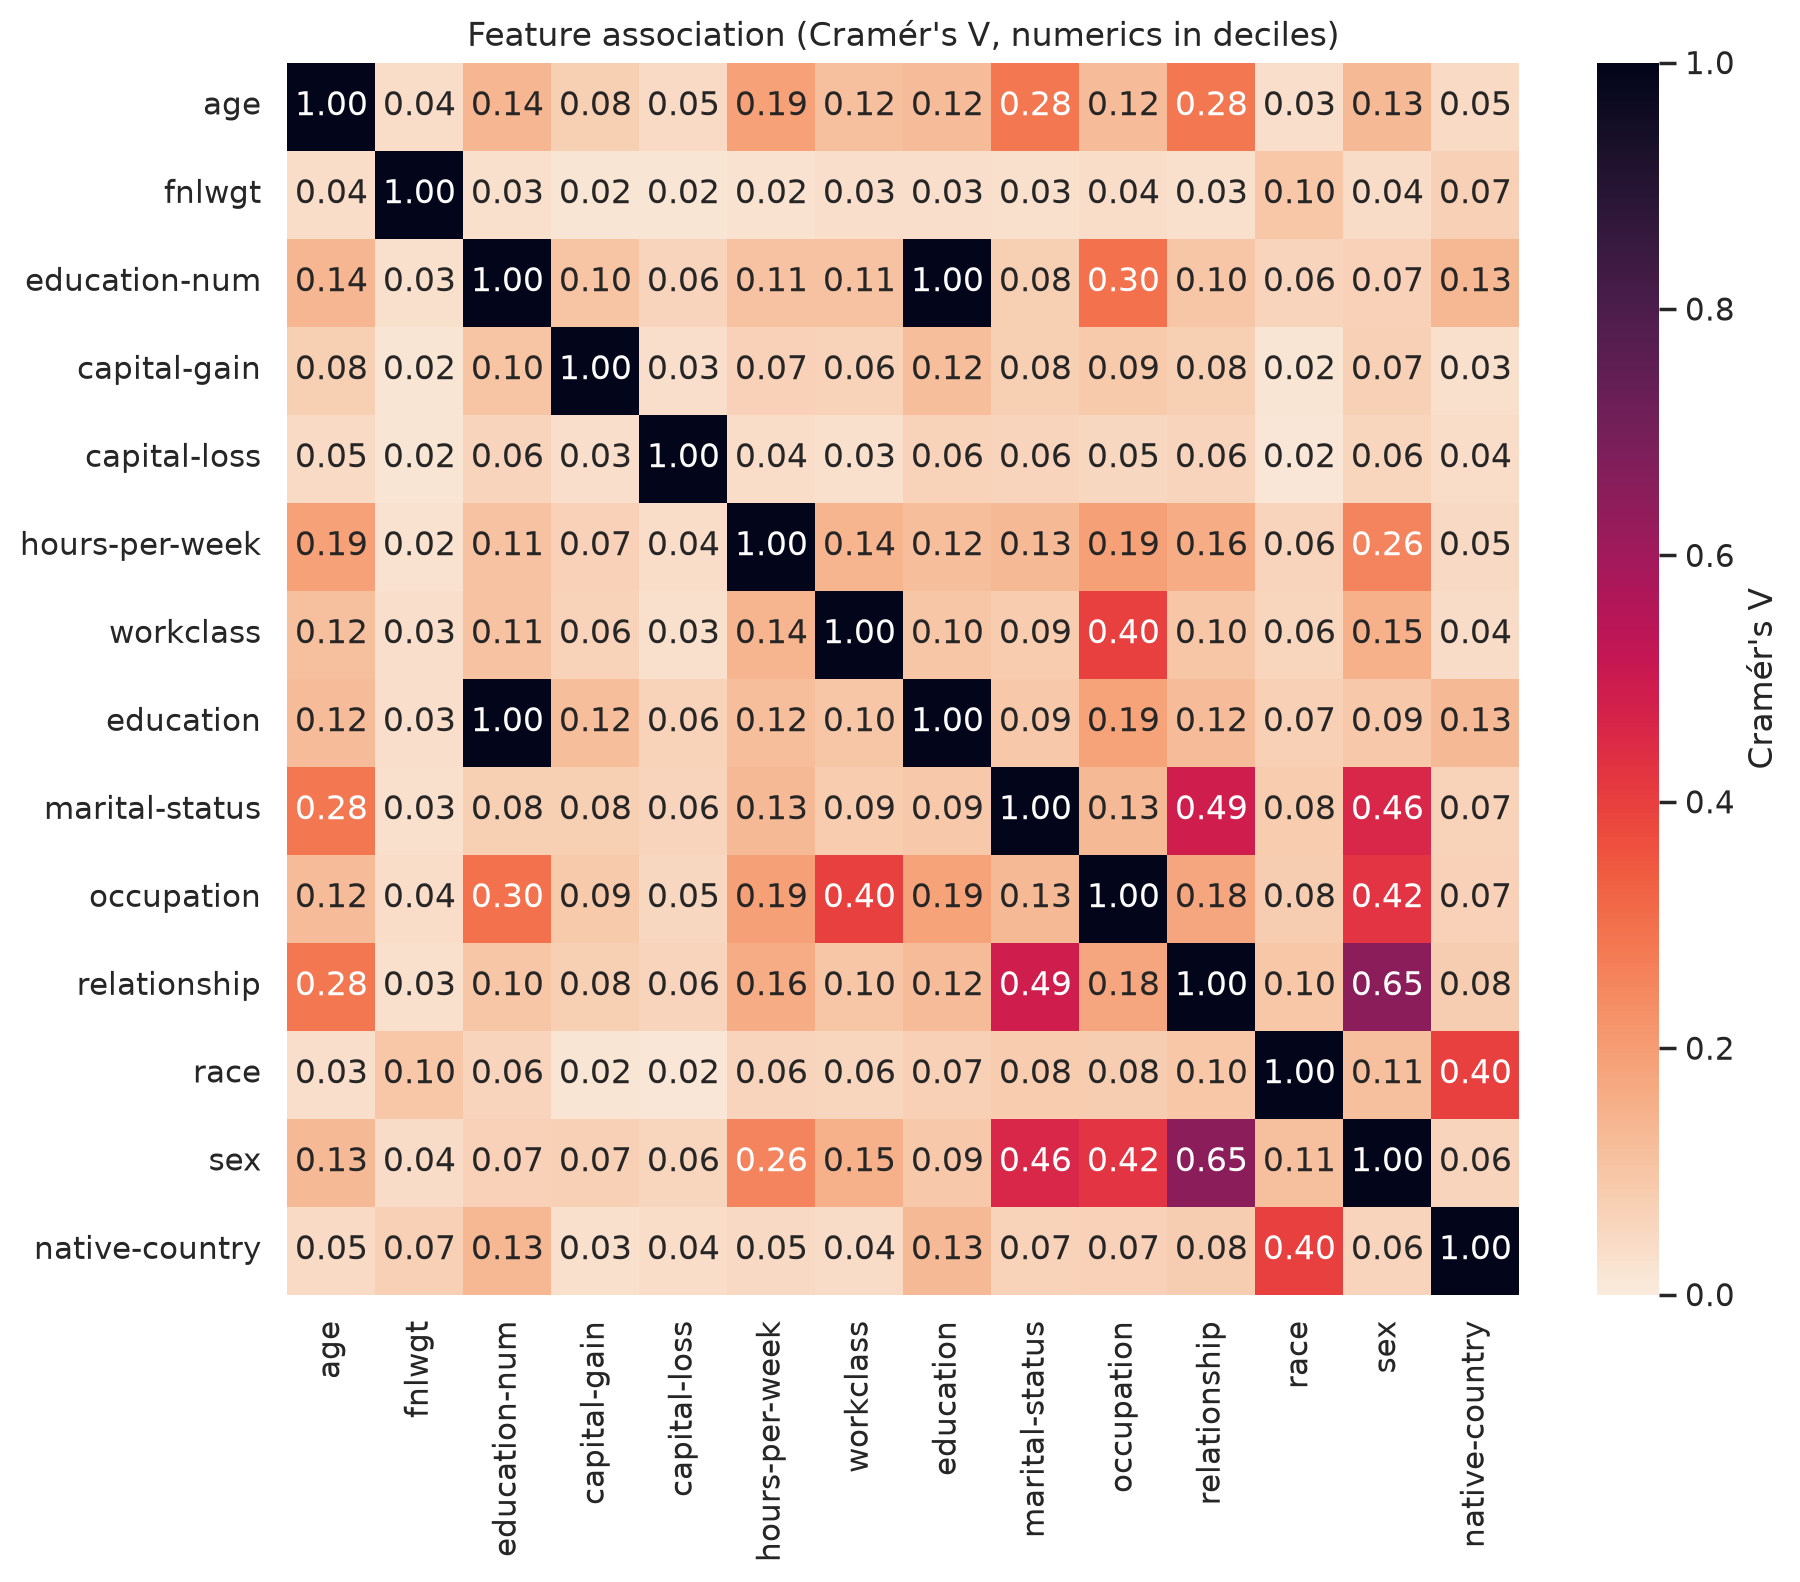
\includegraphics[width=\textwidth]{eda_cramers_v.png}
    \caption{Cram\'er's $V$ between features.}
  \end{subfigure}\hfill
  \begin{subfigure}[b]{0.46\textwidth}
    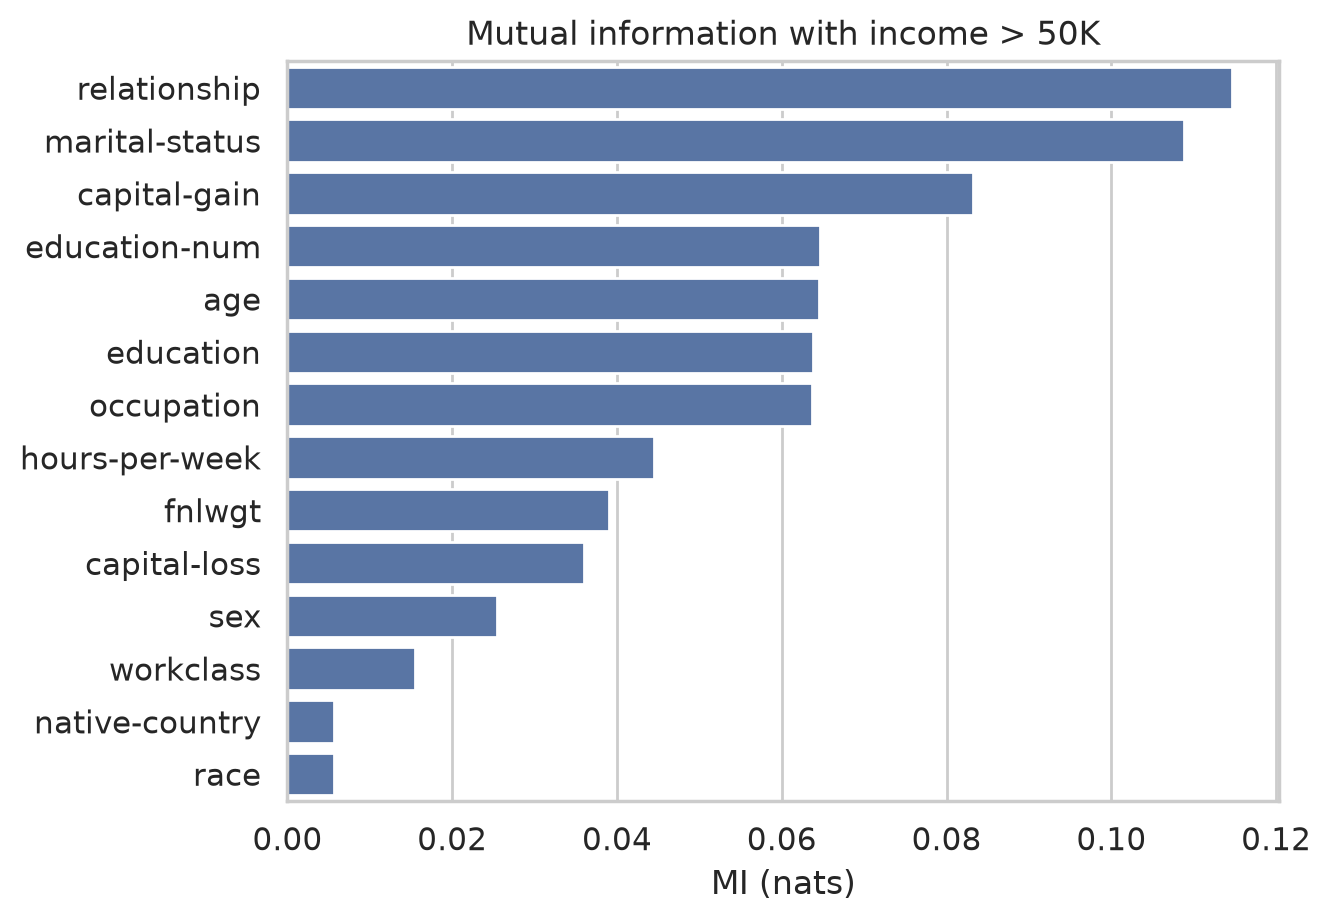
\includegraphics[width=\textwidth]{eda_mutual_information.png}
    \caption{Mutual information with the target.}
  \end{subfigure}
  \caption{EDA evidence used to build the ontology.}
  \label{fig:eda}
\end{figure}

We also examined value-level groupings of high-cardinality columns (e.g.\ WhiteCollar / BlueCollar / Service for
\code{occupation}; BelowHighSchool \dots\ Postgraduate for \code{education}). Several groups are not homogeneous
(\code{Adm-clerical} has a positive rate of 0.14 inside WhiteCollar; \code{Self-emp-inc} 0.55 vs.\
\code{Self-emp-not-inc} 0.28), so they were \emph{not} turned into sub-concepts; they only support that each
feature forms a meaningful leaf concept.

%=====================================================================
\section{Ontology}\label{sec:ontology}
%=====================================================================

The ontology (\cref{fig:ontology}) has a root \concept{Person}, five top-level concepts (level~1) and ten leaf
concepts (level~2). Each leaf is linked to its source features with an OWL annotation property
\code{mapsToFeature}; one-hot columns inherit the concept of their source feature. The file
\code{data/ontology/adult.owl} opens in Prot\'eg\'e, and every lookup in the analysis reads the saved OWL file, so
the analysis depends on the ontology and not on a hard-coded mapping.

\begin{figure}[t]
  \centering
  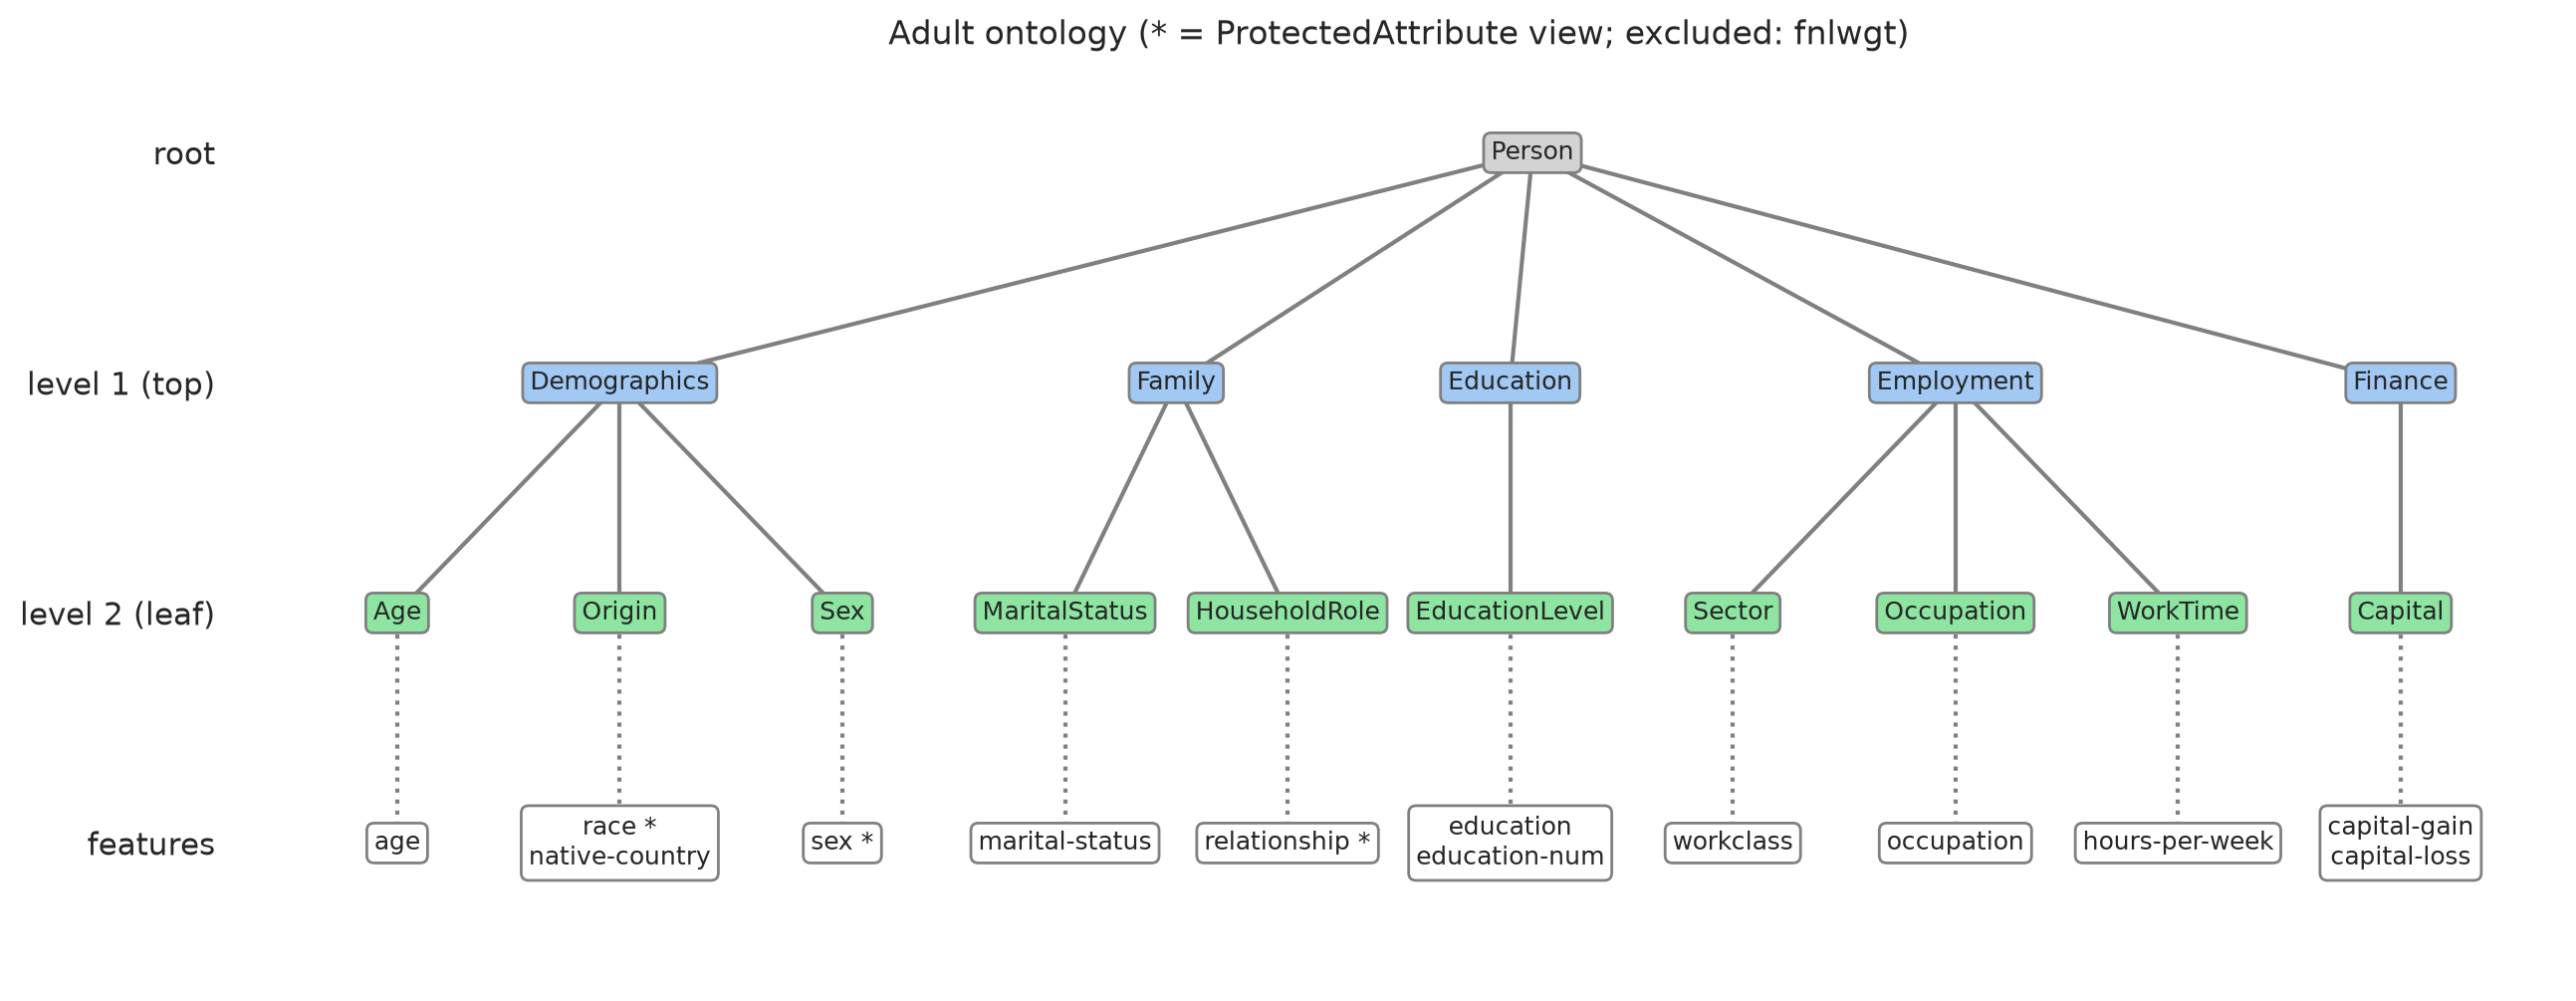
\includegraphics[width=\textwidth]{ontology_hierarchy.png}
  \caption{The Adult ontology: \concept{Person} $\rightarrow$ 5 top concepts $\rightarrow$ 10 leaf concepts.
    \concept{ProtectedAttribute} is a separate view over \code{race}, \code{sex} and \code{relationship}.}
  \label{fig:ontology}
\end{figure}

\begin{table}[t]
  \centering\small
  \caption{Leaf concepts, source features and design rationale.}
  \label{tab:ontology}
  \begin{tabularx}{\textwidth}{@{}llll X@{}}
    \toprule
    Top concept & Leaf concept & Features & Cols & Rationale \\
    \midrule
    \multirow{3}{*}{\concept{Demographics}} & \concept{Age} & age & 1 & separate signal \\
      & \concept{Origin} & race, native-country & 46 & associated, $V=0.40$ \\
      & \concept{Sex} & sex & 2 & separate signal \\
    \midrule
    \multirow{2}{*}{\concept{Family}} & \concept{MaritalStatus} & marital-status & 7 & strongest MI; split so the leaf \\
      & \concept{HouseholdRole} & relationship & 6 & level shows which one is used \\
    \midrule
    \concept{Education} & \concept{EducationLevel} & education, education-num & 17 & same variable ($V=1$) \\
    \midrule
    \multirow{3}{*}{\concept{Employment}} & \concept{Sector} & workclass & 8 & weak MI \\
      & \concept{Occupation} & occupation & 14 & medium MI \\
      & \concept{WorkTime} & hours-per-week & 1 & medium MI \\
    \midrule
    \concept{Finance} & \concept{Capital} & capital-gain, capital-loss & 2 & income from assets \\
    \midrule
    \multicolumn{2}{@{}l}{\concept{ProtectedAttribute} (view)} & race, sex, relationship & 13 & relationship leaks sex \\
    \multicolumn{2}{@{}l}{(excluded)} & fnlwgt & -- & sampling weight \\
    \bottomrule
  \end{tabularx}
\end{table}

Design choices (\cref{tab:ontology}):
\begin{itemize}
  \item \textbf{Two levels only.} Level~2 is fine enough to show \emph{which} of two correlated features a member
    uses; level~1 shows whether members agree on the broader idea. Value-level sub-concepts were rejected (see
    \cref{sec:data}).
  \item \textbf{\concept{ProtectedAttribute} as a separate view.} It sits outside \concept{Person}, so every
    feature keeps exactly one leaf and one top concept; the view is used only to report how much the members rely
    on protected attributes and their proxy.
  \item \textbf{Features outside the ontology} (\code{fnlwgt}) are removed from the model inputs, as in TREPAN
    Reloaded~\cite{confalonieri2021trepan}. The encoded design matrix has 104 columns from 13 features.
  \item \textbf{Information content.} Following TREPAN Reloaded we compute the intrinsic IC of Seco et
    al.~\cite{seco2004ic}, $\mathrm{IC}(c) = 1 - \log(\mathrm{sub}(c)+1)/\log N$ with $N = 16$ concepts under
    \concept{Person}. Leaves have IC 1, \concept{Person} 0; among top concepts, \concept{Education} and
    \concept{Finance} (0.75) rank as more specific than \concept{Family} (0.60), \concept{Demographics} and
    \concept{Employment} (0.50). IC is reported only; it is not used for training or weighting.
\end{itemize}

%=====================================================================
\section{Method}\label{sec:method}
%=====================================================================

\subsection{Ensembles}
Both ensembles are trained on the same 104-column training matrix with \code{random\_state=42}.

\begin{description}
  \item[RF] \code{RandomForestClassifier}~\cite{breiman2001rf}: 100 trees, \code{max\_depth=5},
    \code{max\_features=0.3} per split. A first attempt with depth~4 and the default $\sqrt{d}$ features
    ($\approx 10$ of 104 columns per split) gave many members that almost never predicted \texttt{>50K}; the
    chosen setting makes tree members as strong as the LR members.
  \item[LR] \code{BaggingClassifier}~\cite{breiman1996bagging} of 100 pipelines
    \code{StandardScaler} + \code{LogisticRegression}, \code{max\_features=0.5}: each member sees a bootstrap sample and a
    random half of the columns (random patches~\cite{louppe2012patches}). Without feature subsampling, bagged
    linear models converge to nearly the same model and agreement would be trivial. The scaler sits inside each
    member so that coefficients are comparable across features and on the member's own data.
\end{description}

\subsection{Per-member contributions}
For a member $m$, sample $x$ and encoded column $f$ we compute a contribution $\phi_m(x,f)$ in class-1 log-odds,
so both member types share one scale.

\paragraph{Tree members (Saabas path decomposition~\cite{saabas2014}).}
Let $p(n)$ be the class-1 probability at node $n$, Laplace-smoothed as $\tilde p(n) = (p\,w_n + 1)/(w_n+2)$ with
$w_n$ the bootstrap-weighted sample count, so pure nodes stay finite. With
$\ell(n) = \log \tilde p(n) / (1-\tilde p(n))$, every edge parent $\to$ child carries the credit
$\ell(\text{child}) - \ell(\text{parent})$, booked on the parent's split feature. Summing the credits along the
decision path of $x$ gives
\begin{equation}
  \sum_f \phi_m(x,f) = \ell_m(\text{leaf}(x)) - \ell_m(\text{root}).
\end{equation}
The implementation builds a sparse (nodes $\times$ features) credit matrix and multiplies it by sklearn's
\code{decision\_path} indicator matrix. This helper is the only algorithm written by hand: sklearn exposes the
tree structure but not path contributions.

\paragraph{LR members.}
On standardised inputs $z$ the contribution is $\phi_m(x,f) = \beta_{m,f}\, z_f$, i.e.\
$\beta_f (x_f - \mu_f)/\sigma_f$, so $\sum_f \phi_m(x,f) = \ell_m(x) - \ell_m(\mu)$. Columns outside the
member's subset get 0.

Both decompositions are exact: on the full test set the maximum deviation from the expected sums is
$8.4\times10^{-7}$ (RF) and $1.2\times10^{-5}$ (LR), i.e.\ float32 rounding. The total $\sum_f|\phi|$ per member
and sample has a median of 2.7 (RF) and 4.0 (LR) log-odds: the same order of magnitude.

\subsection{Concept vectors}
For a concept $k$ at a given level, the concept vector of member $m$ on sample $x$ is
\begin{equation}
  c_m(x,k) = \frac{\sum_{f \in k} |\phi_m(x,f)|}{\sum_{k'} \sum_{f \in k'} |\phi_m(x,f)|}.
\end{equation}
Absolute values are used because a concept matters to a member whether it pushes towards \texttt{>50K} or away
from it. Vectors are computed at the top level (5 concepts), the leaf level (10 concepts) and for the protected
view (\concept{ProtectedAttribute} vs.\ \concept{Other}). Because contributions are summed, the number of one-hot
columns of a concept (46 for \concept{Origin}, 1 for \concept{Age}) does not by itself inflate it.

\subsection{Metrics}
\paragraph{Agreement (RQ1, RQ3).} For each test sample, over the 100 members:
\begin{itemize}
  \item \textbf{top-concept agreement}: share of members whose top concept ($\arg\max_k c_m(x,k)$) equals the most
    common one (1 = all agree);
  \item \textbf{normalised entropy} of the members' top-concept distribution, divided by $\log K$ so the two levels
    are comparable (0 = all agree);
  \item \textbf{mean pairwise Kendall $\tau_b$}~\cite{kendall1945ties} between the members' concept vectors over
    all $\binom{100}{2}=4950$ pairs (1 = same ranking of all concepts). It is computed without a loop over pairs:
    $\tau_b$ is the cosine between sign vectors $\mathrm{sign}(c_i - c_j)$, and the sum of all pairwise cosines
    of unit vectors equals $(\|\sum u\|^2 - \sum\|u\|^2)/2$.
\end{itemize}
A \emph{shuffled} chance reference permutes each member's concept vector at random per sample, keeping the
values but destroying which concept they belong to.

\paragraph{Disagreement (RQ2).} Member vote $= [\,p_m(x) > 0.5\,]$. The vote margin is
$|\,\text{share voting 1} - \text{share voting 0}\,|$ (0 = split vote, 1 = unanimous). Samples with margin $< 0.2$
are \emph{contested}. For each contested sample the \textbf{camp difference} is the mean concept vector of the
members voting \texttt{>50K} minus that of the members voting \texttt{<=50K} (positive = the \texttt{>50K} camp
weighs the concept more). We also correlate the margin with each agreement metric over the test set (Spearman).

\paragraph{Faithfulness.} For each member and leaf concept, all columns of the concept are permuted together
with one shared row permutation (so one-hot groups stay valid) and the member's accuracy drop is measured. A
faithful attribution should rank concepts like the drops: per member we compute the Spearman correlation between
its 10 mean concept shares and its 10 drops.

%=====================================================================
\section{Results}\label{sec:results}
%=====================================================================

\subsection{Ensembles}

\begin{table}[h]
  \centering\small
  \caption{Test performance and member diversity. Majority baseline accuracy 0.764.}
  \label{tab:ens}
  \begin{tabular}{@{}lccccc@{}}
    \toprule
    & Accuracy & F1 & Mean member F1 & Mean pairwise disagreement & Unanimous samples \\
    \midrule
    RF & 0.852 & 0.625 & 0.58 & 0.07 & 62\,\% \\
    LR & 0.850 & 0.629 & 0.58 & 0.10 & 51\,\% \\
    \bottomrule
  \end{tabular}
\end{table}

Both ensembles perform almost identically and their members are equally strong (\cref{tab:ens},
\cref{fig:members}), so differences in concept agreement are not explained by member quality. Members disagree on
7\,\% (RF) and 10\,\% (LR) of samples on average~\cite{kuncheva2003diversity}: enough diversity that concept
agreement is not trivial. At feature level, both ensembles lean most on \code{marital-status} and
\code{relationship}; RF relies more on \code{education-num}, \code{capital-gain} and \code{age}, while LR spreads
weight over \code{occupation}, \code{education}, \code{sex}, \code{workclass} and \code{native-country}.

\begin{figure}[h]
  \centering
  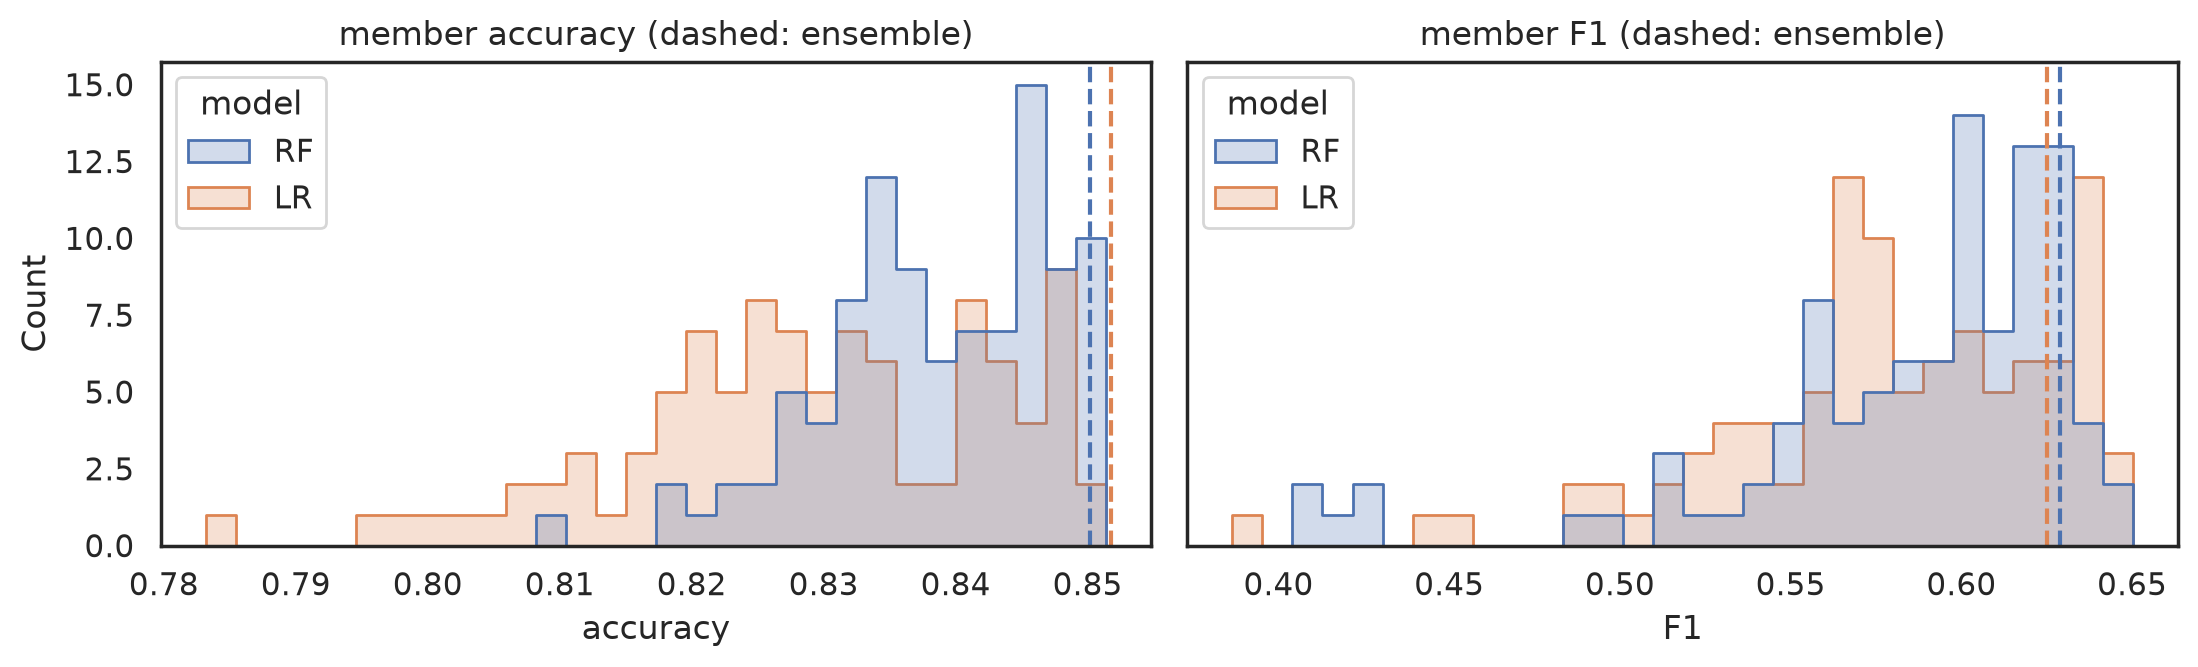
\includegraphics[width=\textwidth]{member_performance.png}\\[4pt]
  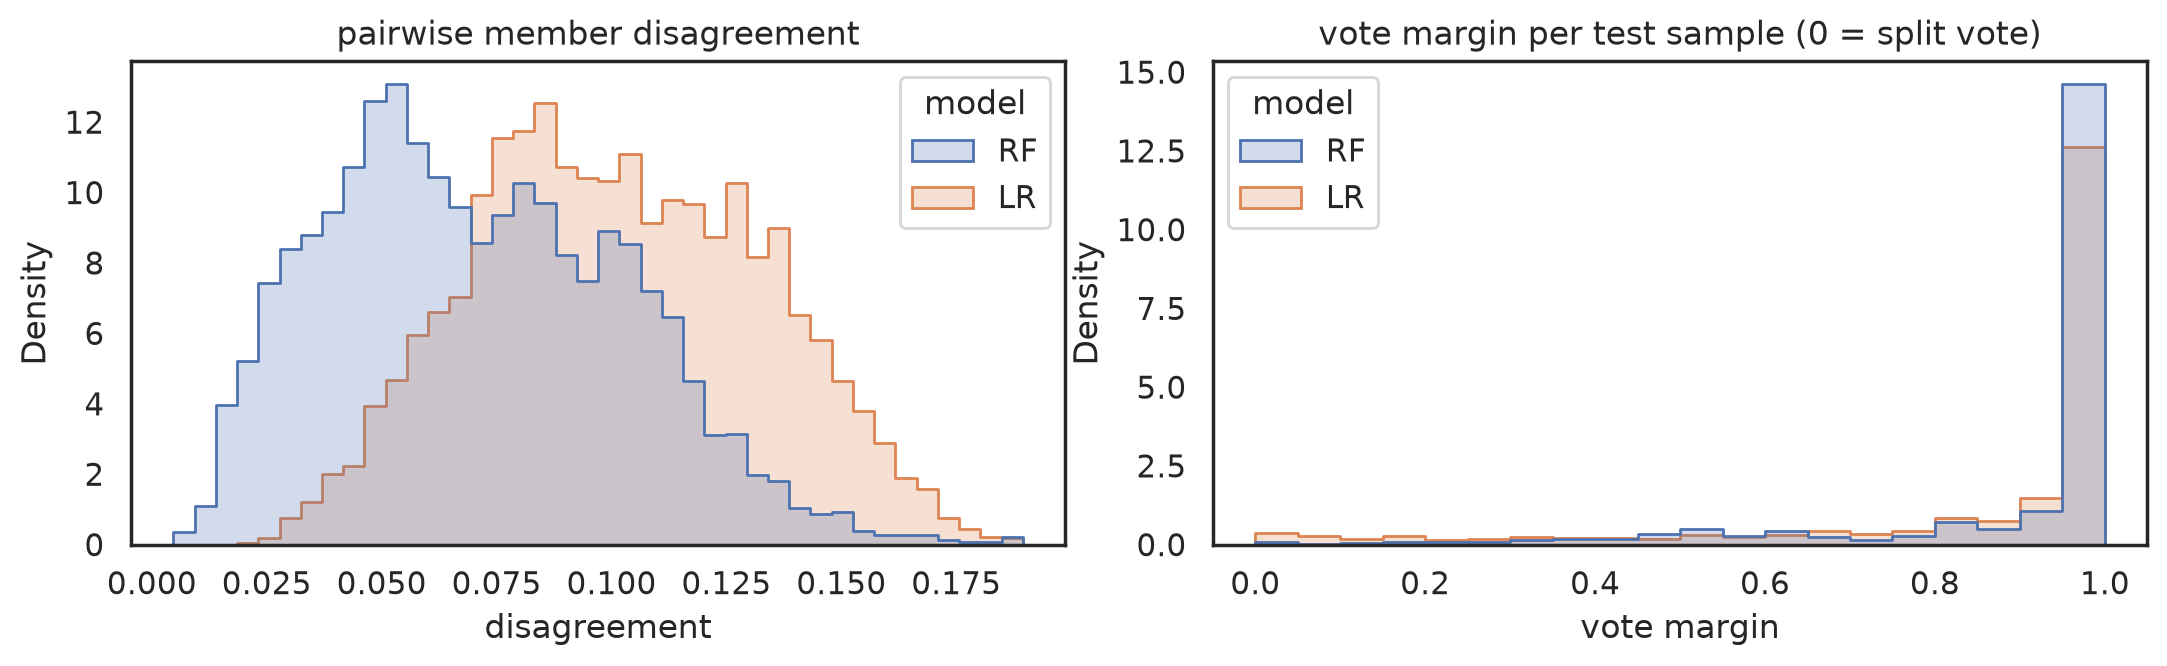
\includegraphics[width=\textwidth]{member_diversity.png}
  \caption{Top: single-member accuracy and F1 against the ensemble. Bottom: pairwise prediction disagreement
    between members.}
  \label{fig:members}
\end{figure}

\subsection{RQ1 -- Concept agreement}

\begin{table}[h]
  \centering\small
  \caption{Mean agreement over the test set; chance values from the shuffled reference in parentheses.}
  \label{tab:rq1}
  \begin{tabular}{@{}llccc@{}}
    \toprule
    Level & Ensemble & Top-concept agreement & Normalised entropy & Kendall $\tau_b$ \\
    \midrule
    \multirow{2}{*}{top (5)}  & RF & 0.83 (0.25) & 0.30 (0.99) & 0.41 (0) \\
                              & LR & 0.79 (0.25) & 0.38 (0.99) & 0.48 (0) \\
    \midrule
    \multirow{2}{*}{leaf (10)} & RF & 0.53 (0.15) & 0.45 (0.98) & 0.35 (0) \\
                               & LR & 0.51 (0.15) & 0.50 (0.98) & 0.37 (0) \\
    \bottomrule
  \end{tabular}
\end{table}

\textbf{Members agree far above chance, and agreement is higher at the top ontology level} (\cref{tab:rq1},
\cref{fig:rq1}). Agreement is partial, however: at the leaf level about half of the members name a different
dominant concept than the majority.

The gain at the top level comes mostly from \concept{Family}. The member $\times$ concept heatmap
(\cref{fig:heatmap}) shows that members split into a \concept{MaritalStatus} group and a
\concept{HouseholdRole} group; the two features carry the same signal (married, husband/wife). At the leaf level
the two groups disagree; at the top level both count as \concept{Family}, which is the dominant concept in
76--77\,\% of (member, sample) pairs. \emph{The ontology turns a substitution between correlated features into
agreement on one concept}, which is exactly the kind of abstraction TREPAN Reloaded exploits. The concepts that
dominate (\concept{Family}, \concept{Education}, \concept{Finance}) are the ones the EDA predicted from mutual
information.

\begin{figure}[h]
  \centering
  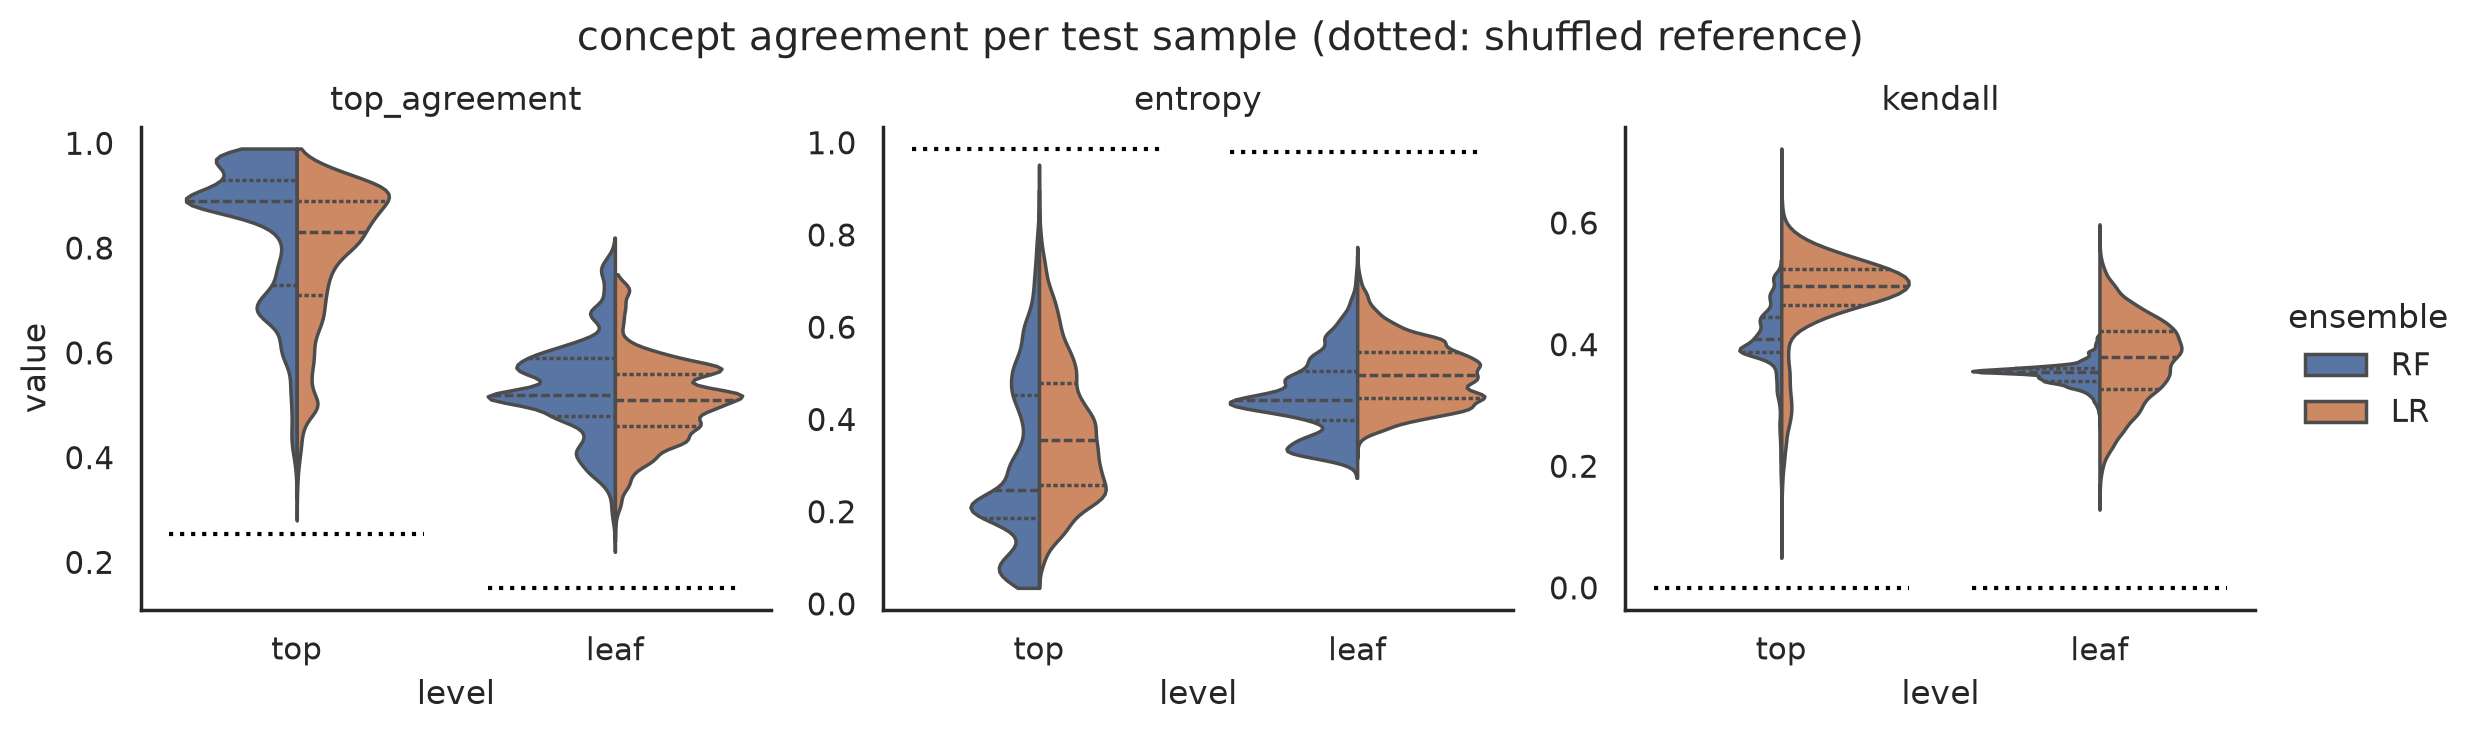
\includegraphics[width=\textwidth]{agreement_by_level.png}\\[4pt]
  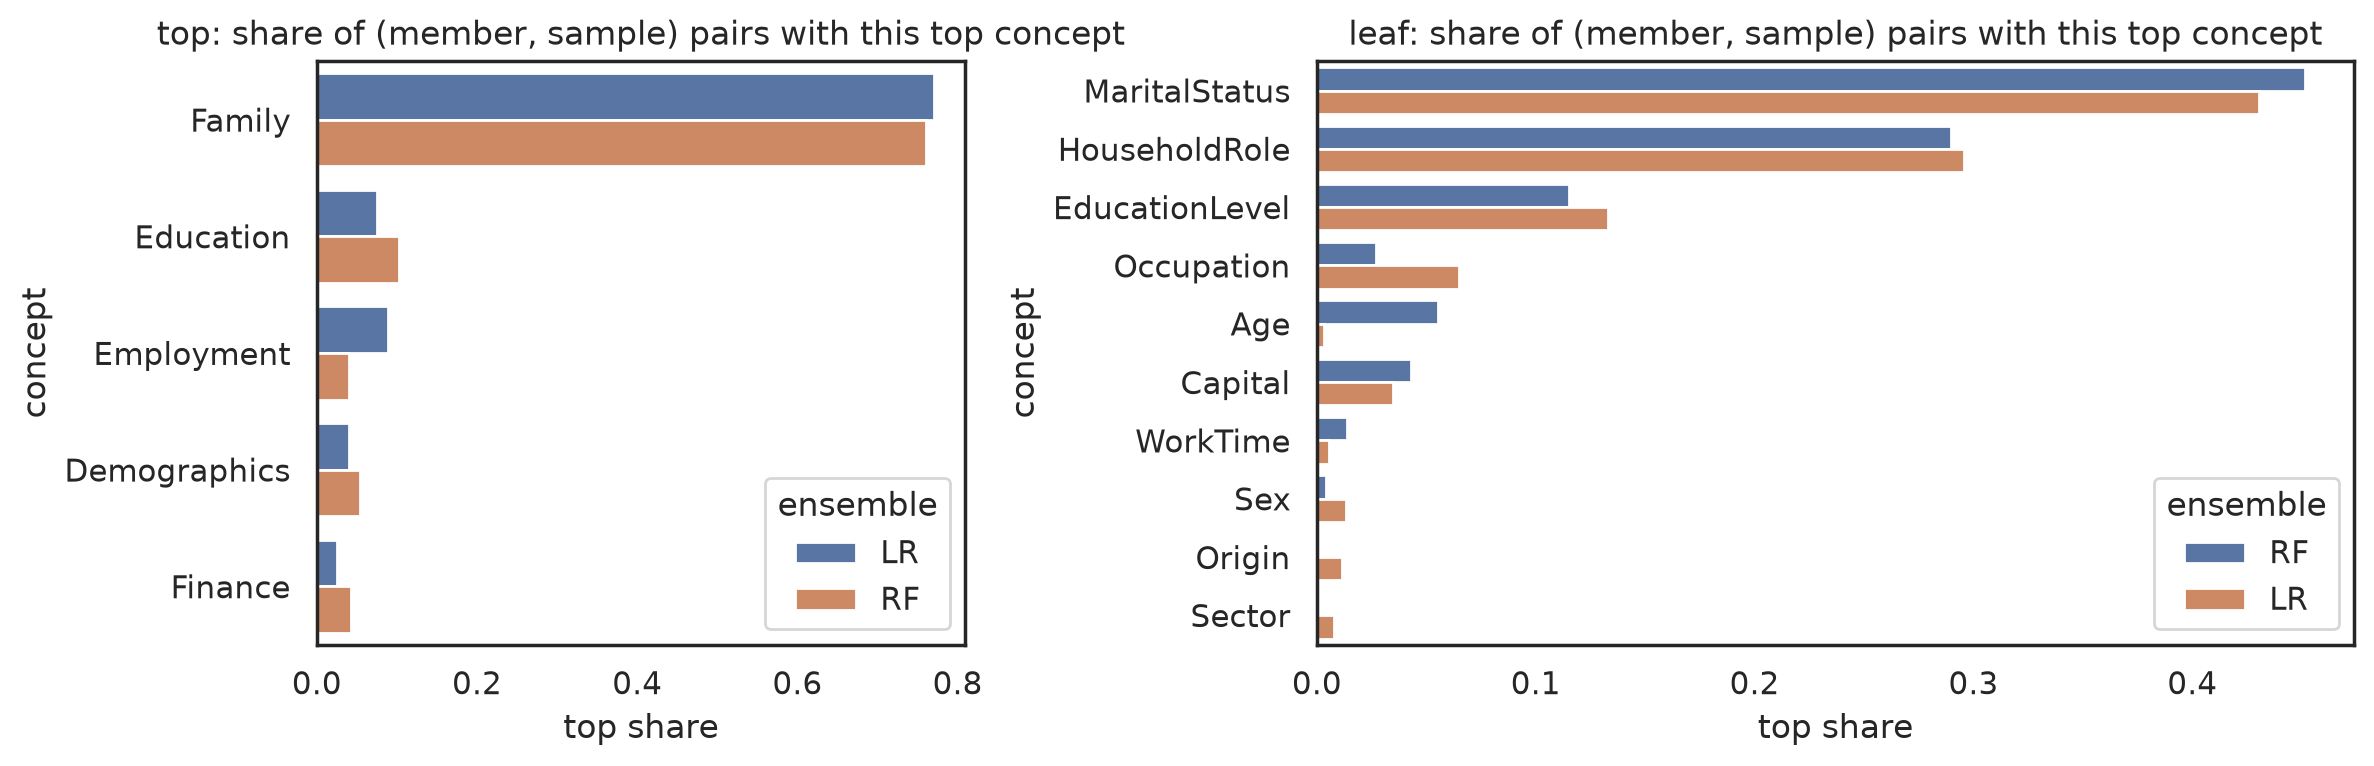
\includegraphics[width=\textwidth]{top_concepts.png}
  \caption{Top: distribution of the three agreement metrics per ensemble and ontology level. Bottom: how often each
    concept is a member's dominant concept.}
  \label{fig:rq1}
\end{figure}

\begin{figure}[h]
  \centering
  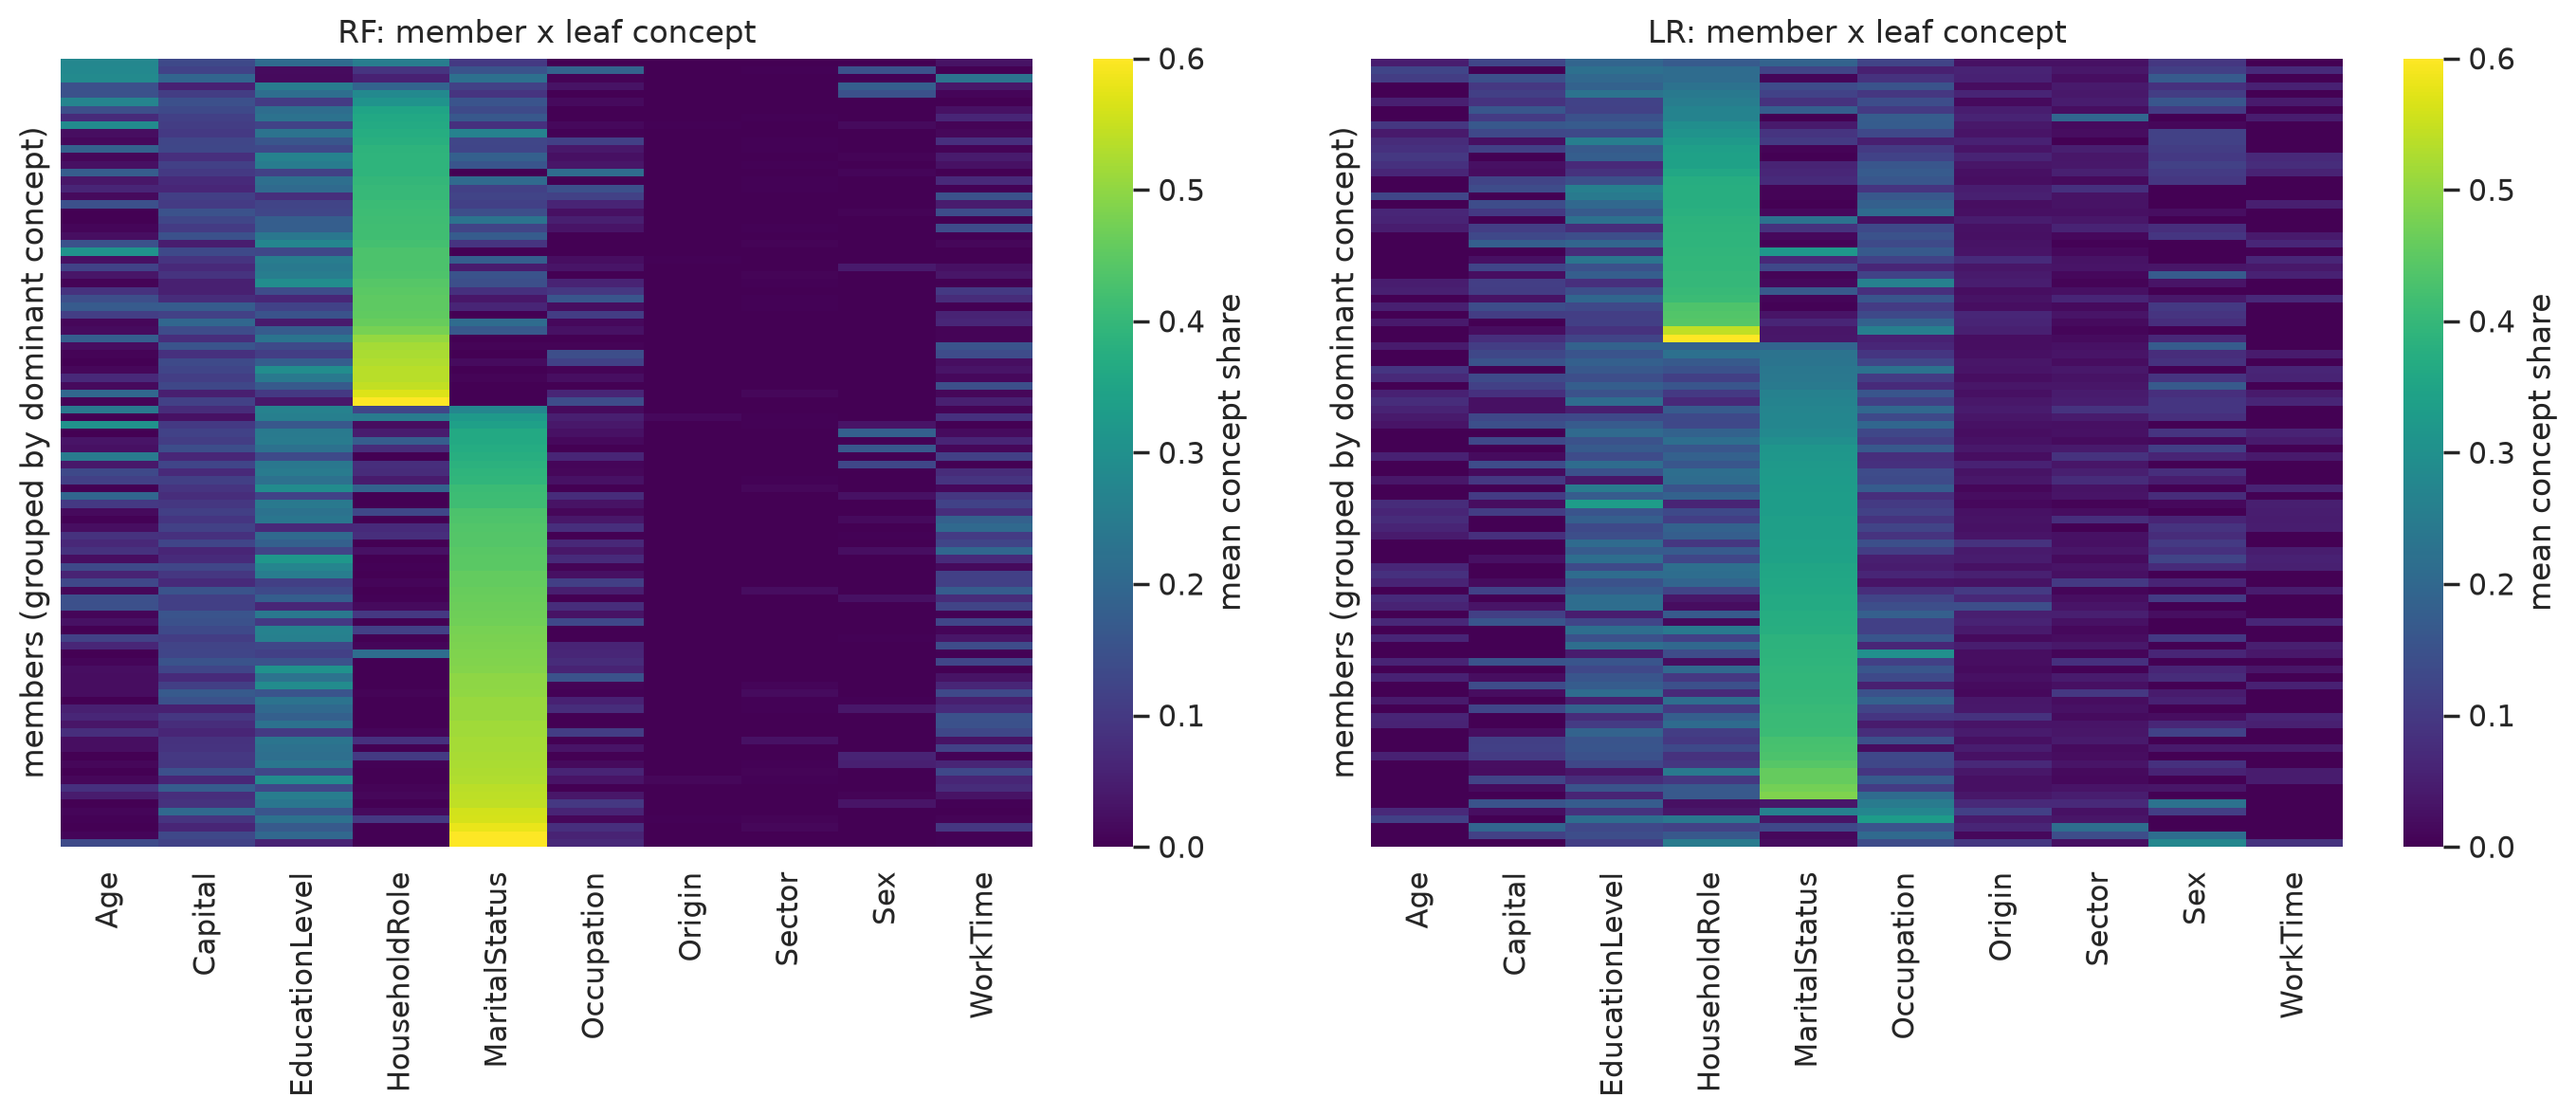
\includegraphics[width=\textwidth]{member_concept_heatmap.png}
  \caption{Mean leaf-concept share per member (rows grouped by dominant concept). Members specialise on either
    \concept{MaritalStatus} or \concept{HouseholdRole}.}
  \label{fig:heatmap}
\end{figure}

\subsection{RQ2 -- Concept disagreement}

\textbf{Prediction disagreement goes with concept disagreement, mostly on which concept dominates.}

\begin{itemize}
  \item Contested samples (margin $< 0.2$) are rare: 190 (RF) and 884 (LR) of 16{,}281.
  \item The vote margin correlates with top-concept entropy at $\rho = -0.63$ (RF, top), $-0.32$ (RF, leaf),
    $-0.39$ / $-0.42$ (LR, top / leaf). For RF at the top level, top-concept agreement falls from 0.89 on unanimous
    samples to 0.51 on contested ones (\cref{fig:margin}).
  \item The link with the full ranking is weak ($\rho$ between margin and Kendall 0.08--0.20,
    \cref{fig:kendallmargin}): members that vote differently still order most concepts alike and differ in which
    concept comes first.
  \item On contested samples the \texttt{>50K} camp is coherent (Kendall 0.47 RF, 0.46 LR vs.\ 0.33 / 0.36 for the
    whole ensemble); the \texttt{<=50K} camp is about as mixed as the whole ensemble (0.33 / 0.39). A
    \texttt{>50K} vote on a borderline sample comes from members reading the same evidence; a \texttt{<=50K} vote
    can come from several directions.
\end{itemize}

\begin{figure}[h]
  \centering
  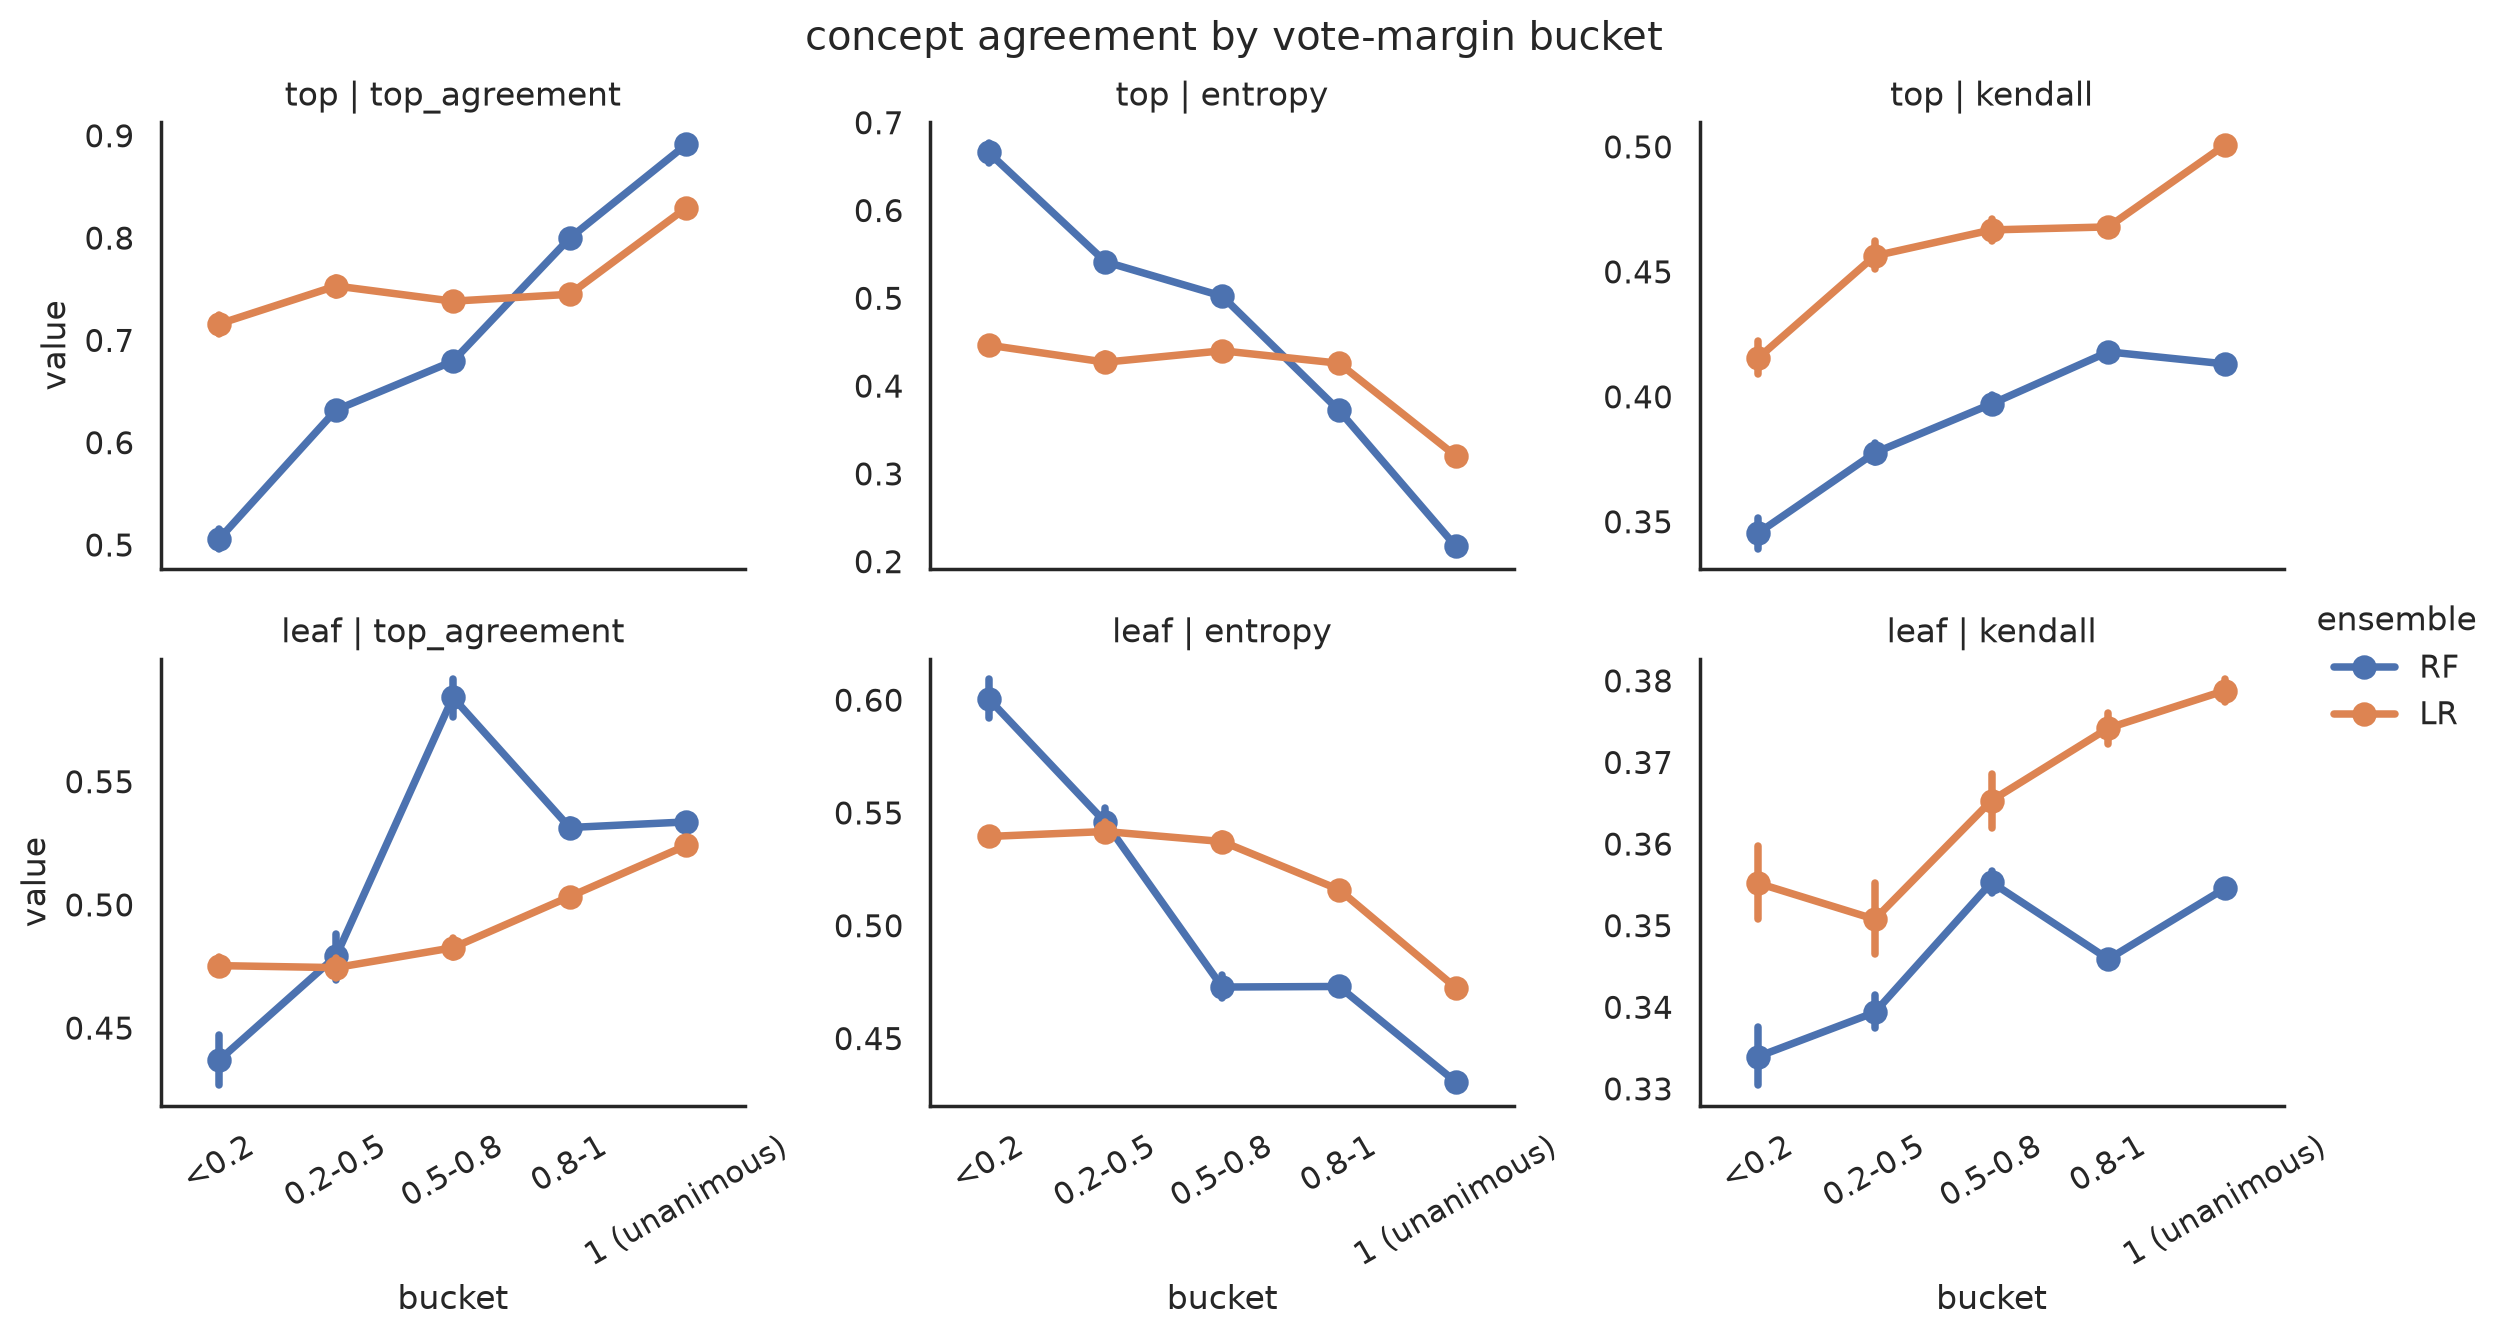
\includegraphics[width=\textwidth]{agreement_by_margin.png}
  \caption{Concept agreement per vote-margin bucket. Concept agreement falls as the vote becomes contested,
    most sharply for RF at the top level.}
  \label{fig:margin}
\end{figure}

\begin{figure}[h]
  \centering
  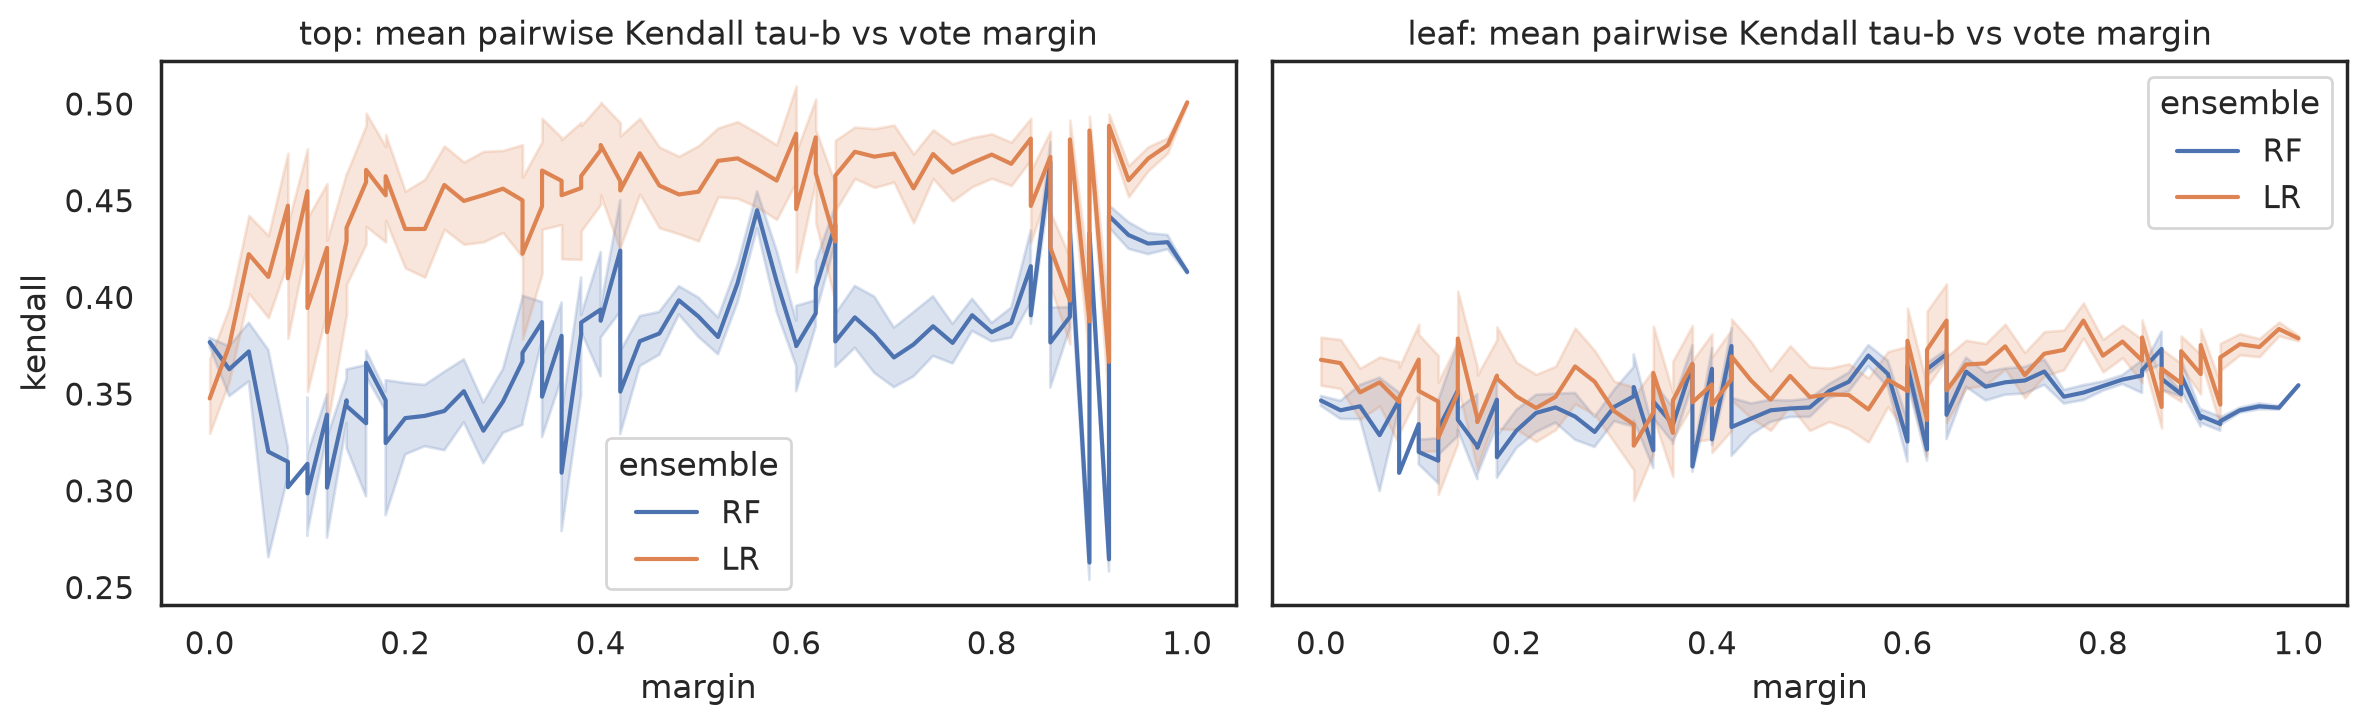
\includegraphics[width=\textwidth]{kendall_vs_margin.png}
  \caption{Vote margin vs.\ mean pairwise Kendall $\tau_b$: only a weak link.}
  \label{fig:kendallmargin}
\end{figure}

\paragraph{Which concepts are read differently.} \Cref{fig:camp} shows the camp difference on contested samples.
The \texttt{>50K} camp weighs \concept{Finance}/\concept{Capital} more ($+0.15$ in both ensembles; in 76\,\% of
contested samples for RF) and, for RF, \concept{EducationLevel} ($+0.08$). The \texttt{<=50K} camp weighs
\concept{Family} more ($-0.11$ RF, $-0.09$ LR), \concept{Demographics}, and for RF \concept{WorkTime} ($-0.10$).
It also uses more \concept{ProtectedAttribute} features ($-0.06$, in 87\,\% of contested samples in both
ensembles).

\begin{figure}[h]
  \centering
  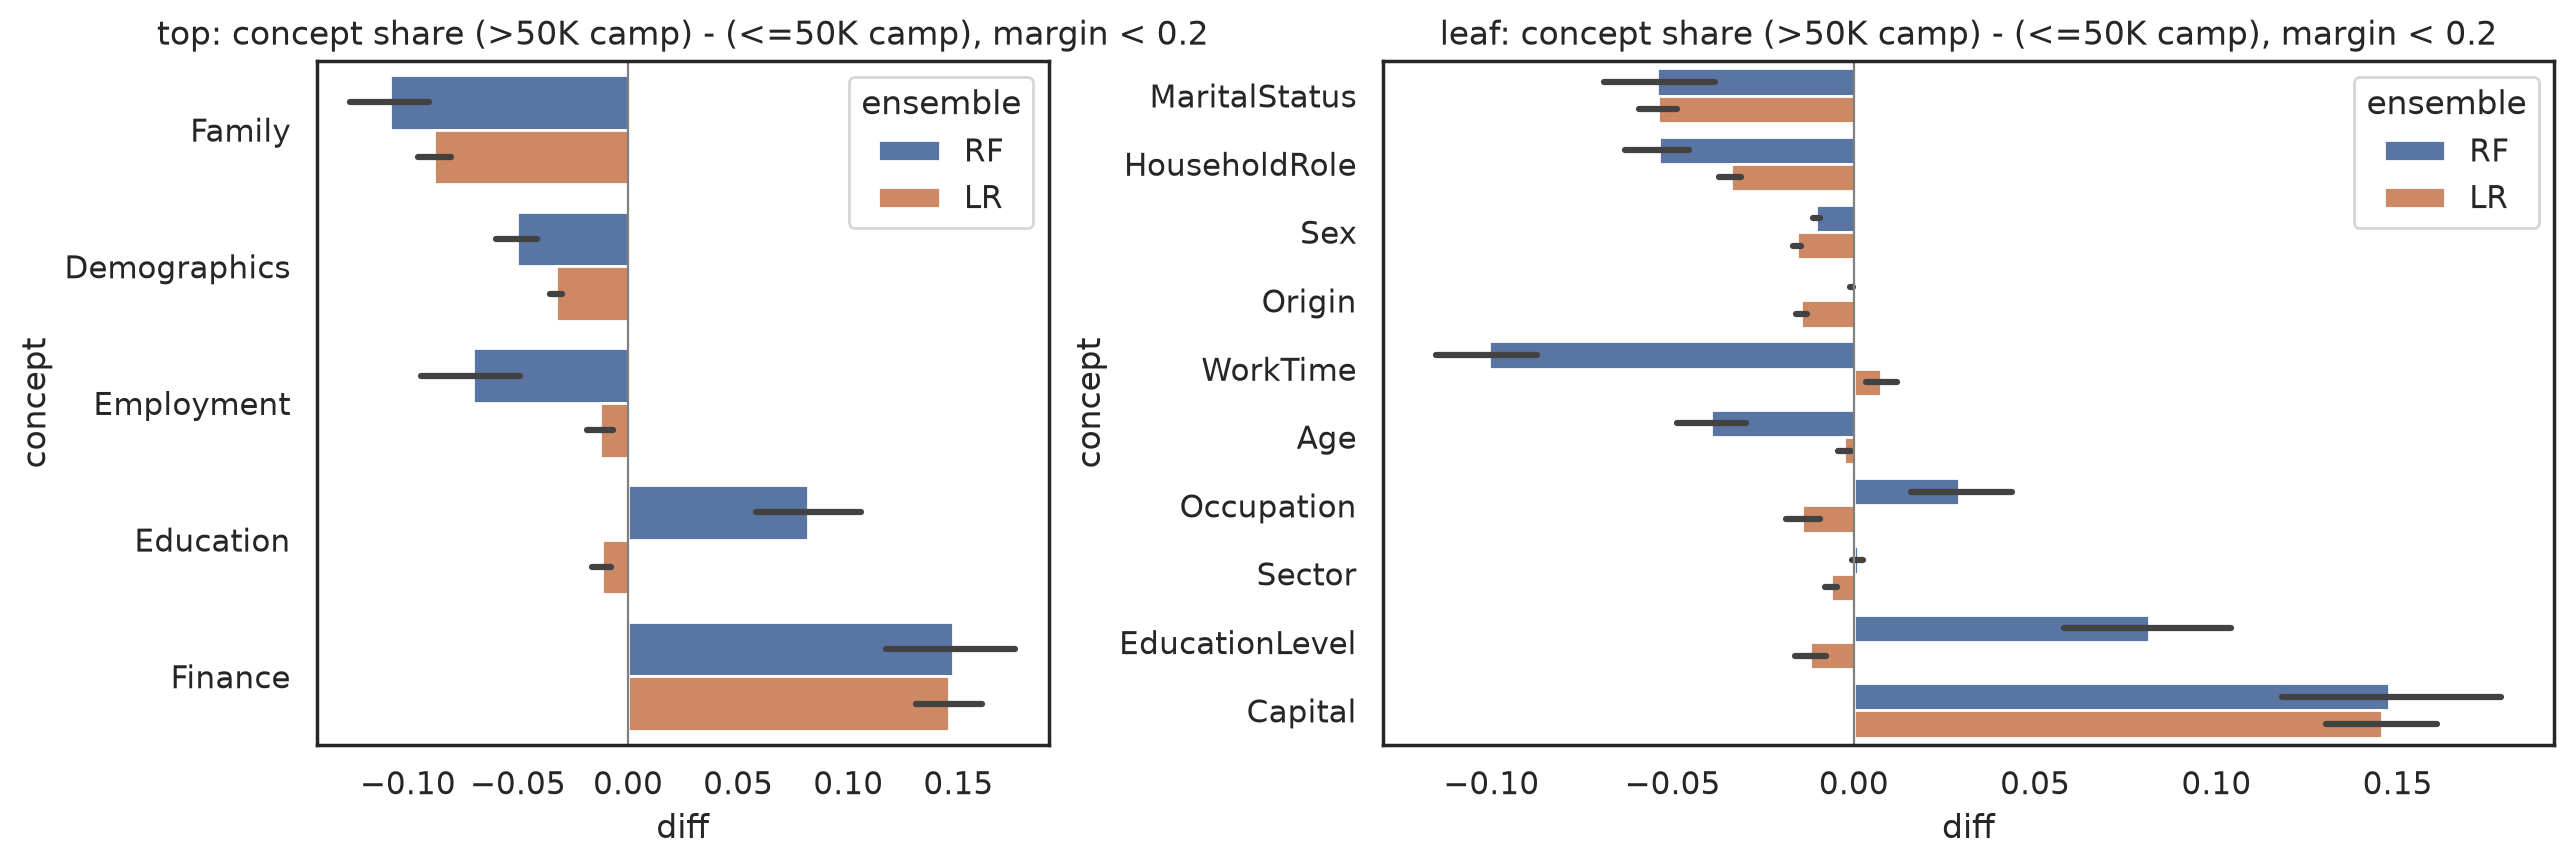
\includegraphics[width=\textwidth]{camp_difference.png}
  \caption{Mean concept vector of the \texttt{>50K} camp minus the \texttt{<=50K} camp on contested samples
    (margin $< 0.2$). Positive = the \texttt{>50K} camp weighs the concept more.}
  \label{fig:camp}
\end{figure}

\paragraph{Case studies.} The four most contested test samples (smallest combined RF + LR margin,
\cref{fig:cases}) are all married, and each pits two strong cues against each other, the same pair in both
ensembles:
\begin{itemize}
  \item \#13037 (true \texttt{>50K}): a 1{,}977 capital loss (\concept{Capital}) vs.\ 10th-grade education
    (\concept{EducationLevel});
  \item \#13211 and \#13135 (true \texttt{<=50K}): a Masters degree (\concept{EducationLevel}) vs.\ only 15 or 4
    working hours per week (\concept{WorkTime});
  \item \#7090 (true \texttt{>50K}): a 5{,}178 capital gain (\concept{Capital}) vs.\ being a wife
    (\concept{HouseholdRole} / \concept{MaritalStatus}).
\end{itemize}
True labels split 2/2, so these are genuine borderline cases and neither camp is simply right. RF camps differ
more sharply than LR camps (camp differences up to 0.59 vs.\ 0.20).

\begin{figure}[h]
  \centering
  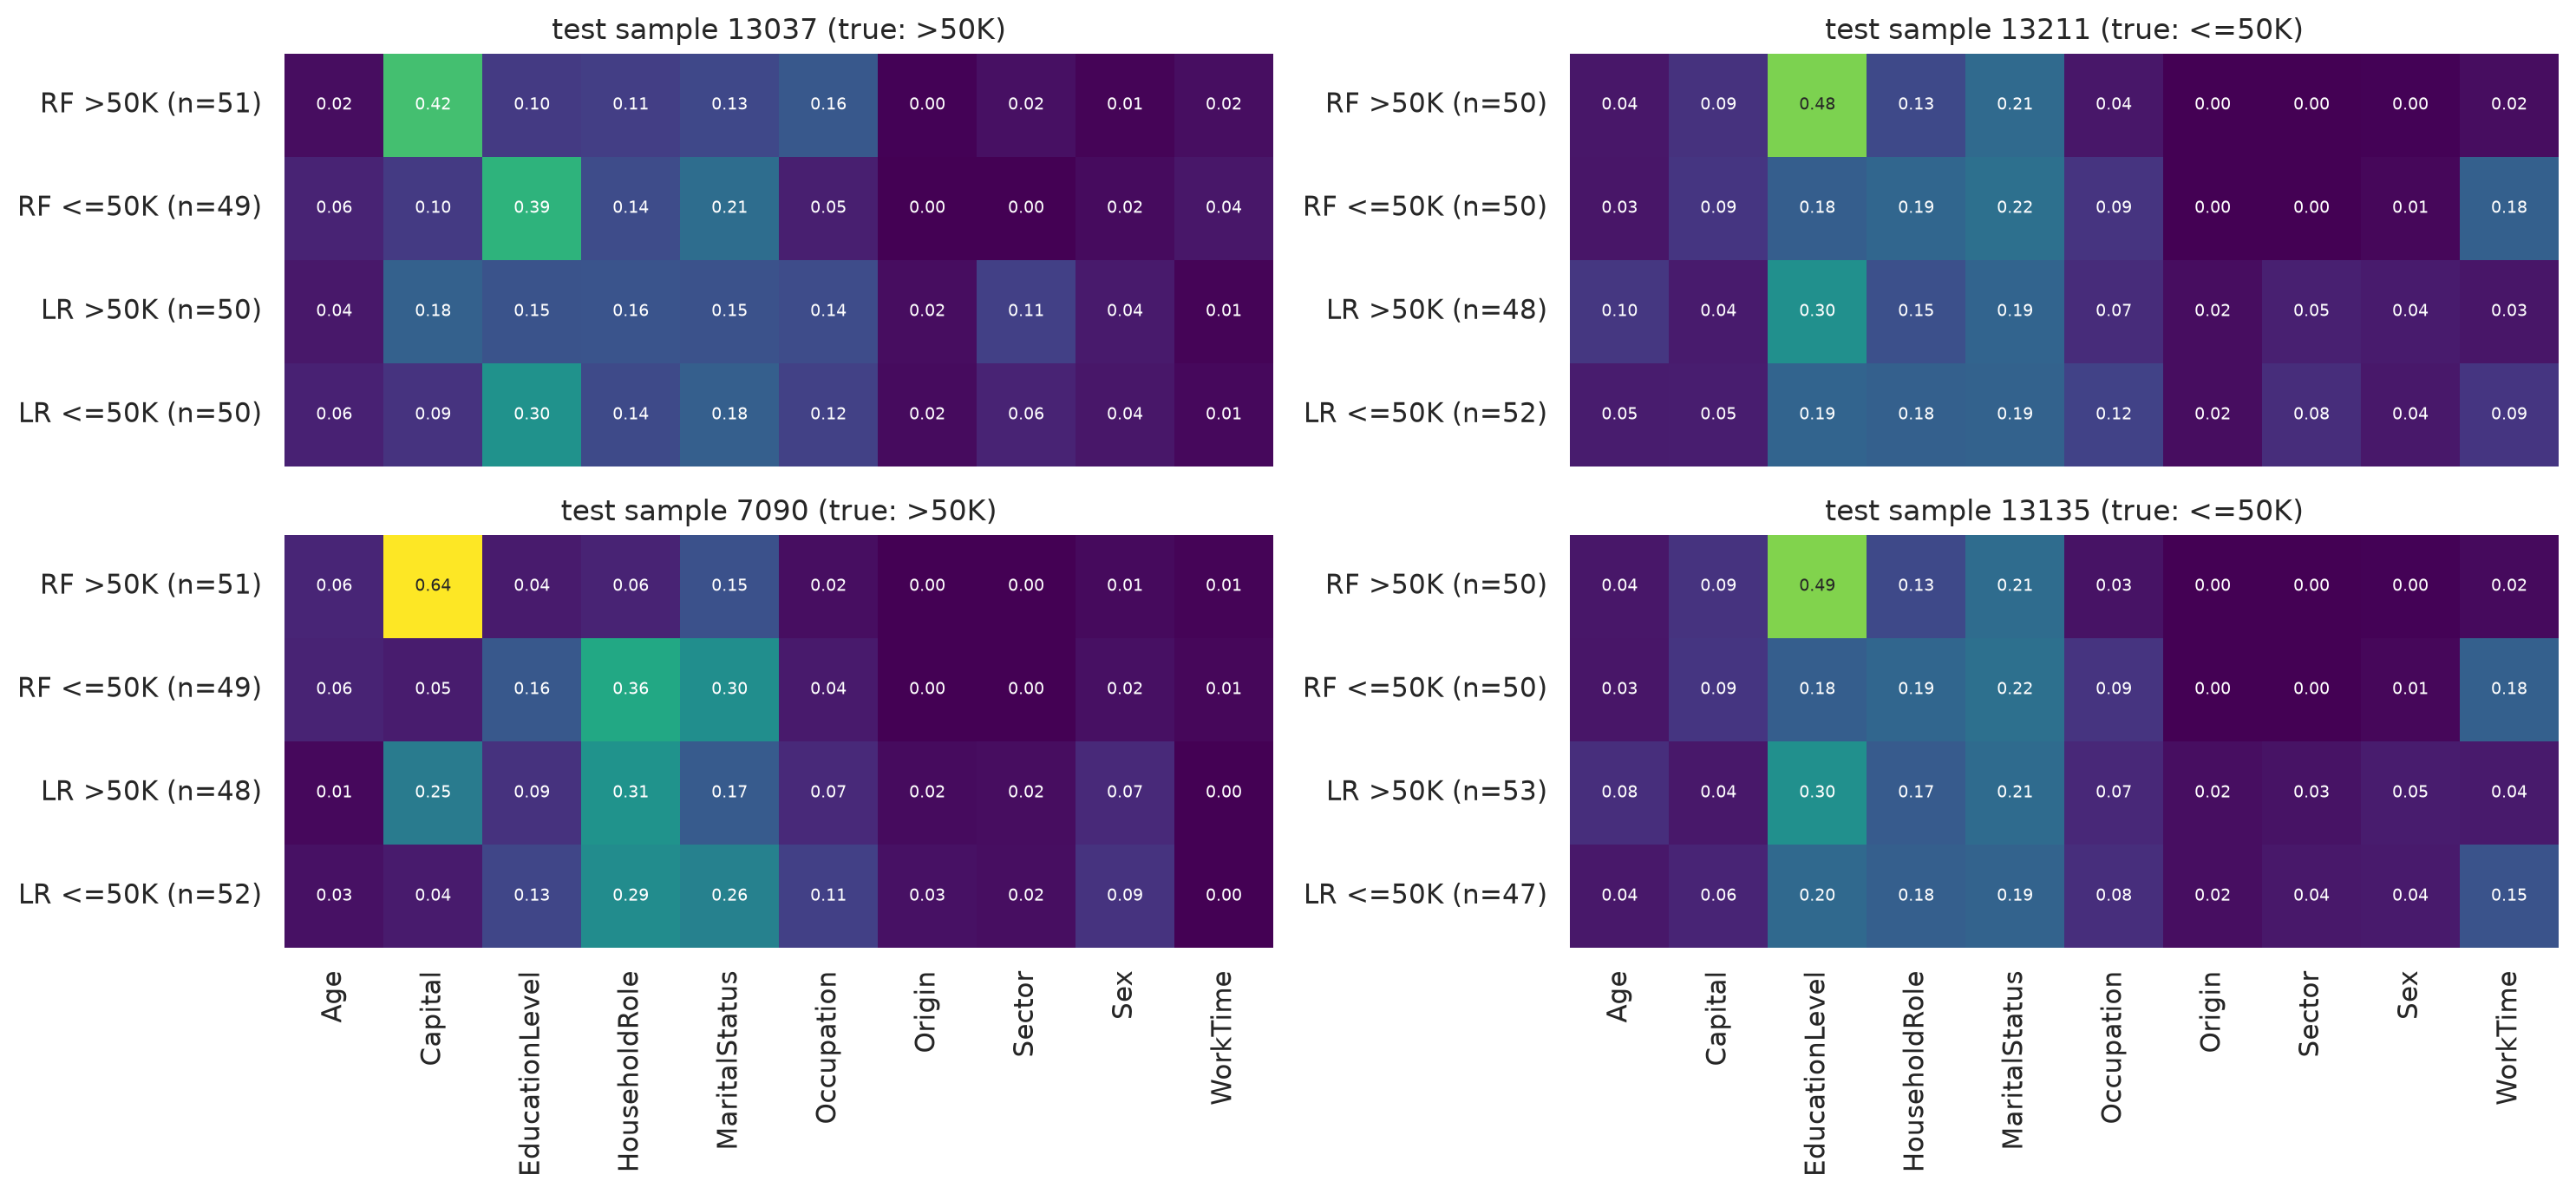
\includegraphics[width=\textwidth]{case_studies.png}
  \caption{Mean leaf concept vector of each voting camp for the four most contested test samples.}
  \label{fig:cases}
\end{figure}

\subsection{RQ3 -- Tree members vs.\ LR members}

\textbf{Trees agree more on the dominant concept; LR members agree more on the full ranking.}
Paired over the same samples, RF has higher top-concept agreement ($+0.05$ top, $+0.03$ leaf) and lower entropy,
but lower Kendall $\tau_b$ ($-0.07$ top, $-0.02$ leaf; LR is higher on 83\,\% of samples at the top level).

The reason is structural. A depth-5 decision path touches at most 5 features, so tree attribution is
concentrated: \concept{Origin}, \concept{Sector} and \concept{Sex} get almost nothing, and the unused concepts
tie, which lowers rank correlation. LR members spread weight over every concept they see (\concept{Occupation}
0.13, \concept{Sex} 0.06, \concept{Origin} and \concept{Sector} 0.04). RF members also specialise more: the
standard deviation across members of the mean share on \concept{HouseholdRole}/\concept{MaritalStatus} is 0.20
vs.\ 0.12--0.16 for LR. Finally, in contested samples RF camps disagree more sharply than LR camps
(\cref{fig:cases}).

\subsection{Protected attributes}
On average 22\,\% (RF) and 30\,\% (LR) of a member's attribution goes to \code{race}, \code{sex} or
\code{relationship}, up to 65--68\,\% for single members; in 17\,\% / 14\,\% of (member, sample) pairs it is more
than half (\cref{fig:protected}). Most of it is \code{relationship} (\concept{HouseholdRole}, a proxy for sex);
LR members also use \code{sex} and \code{race} directly. These features were deliberately kept as model inputs;
the share is reported as a finding, not silently removed.

\begin{figure}[h]
  \centering
  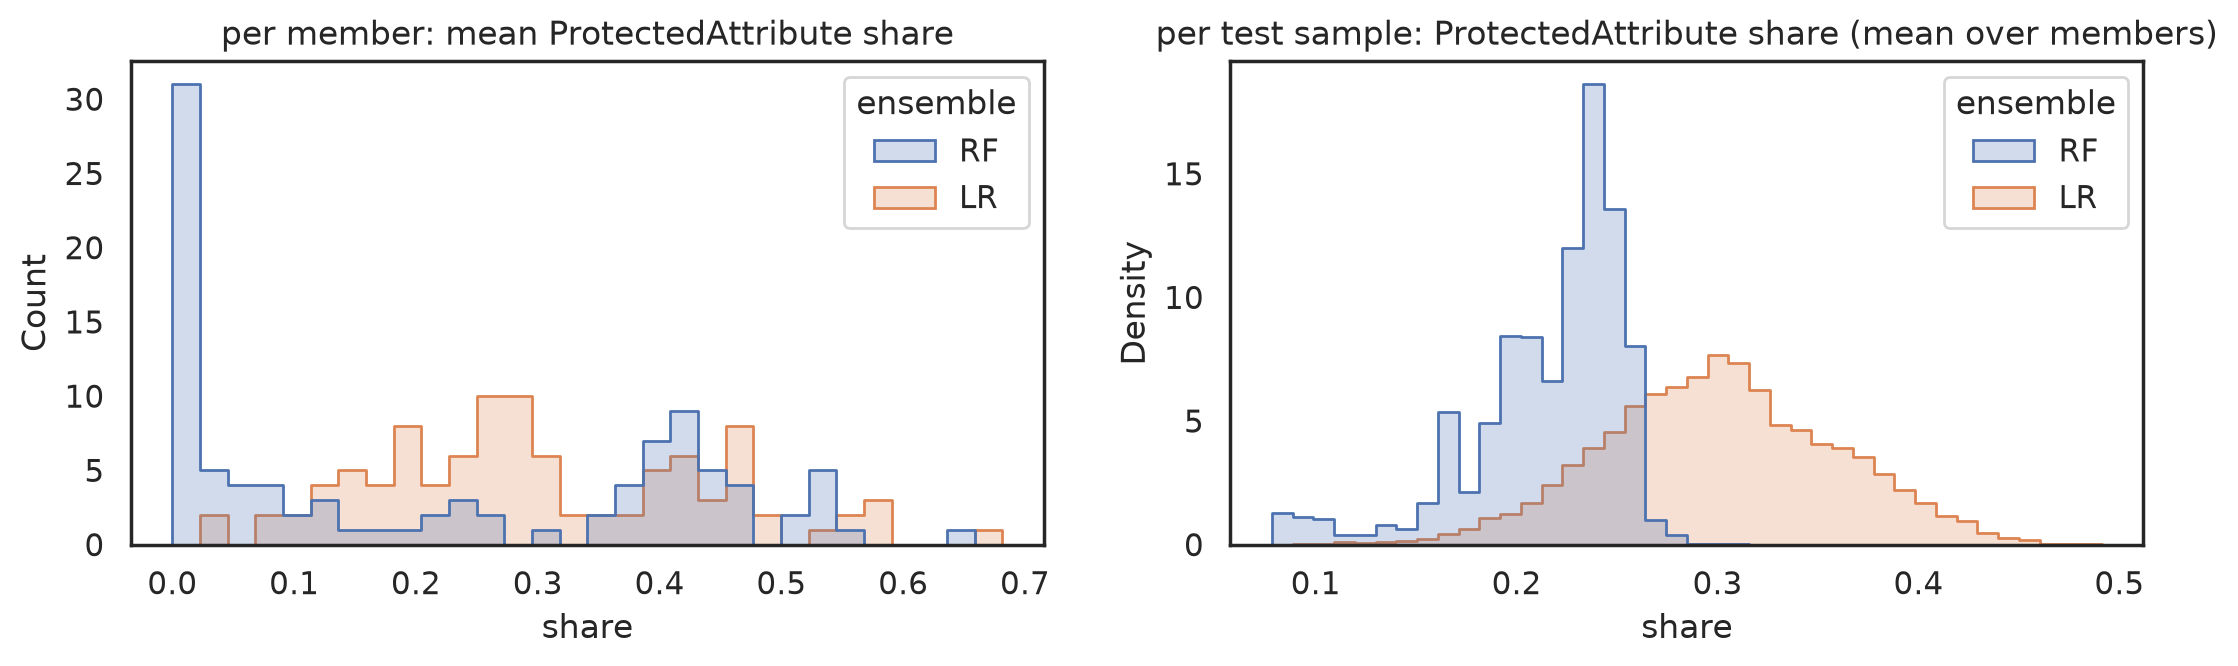
\includegraphics[width=\textwidth]{protected_share.png}
  \caption{Share of each member's attribution on the \concept{ProtectedAttribute} view.}
  \label{fig:protected}
\end{figure}

\subsection{Faithfulness check}
Permuting all columns of one leaf concept ranks concepts like the attribution does: per-member Spearman median
0.78 (RF) and 0.90 (LR), positive for every member (minimum 0.29 / 0.63; \cref{fig:faith}). The main mismatch is
\concept{HouseholdRole}: high attribution but a smaller accuracy drop than \concept{EducationLevel} or
\concept{MaritalStatus}, because \code{marital-status} still carries the signal when \code{relationship} is
permuted. Attribution measures \emph{use}, not \emph{irreplaceability}.

\begin{figure}[h]
  \centering
  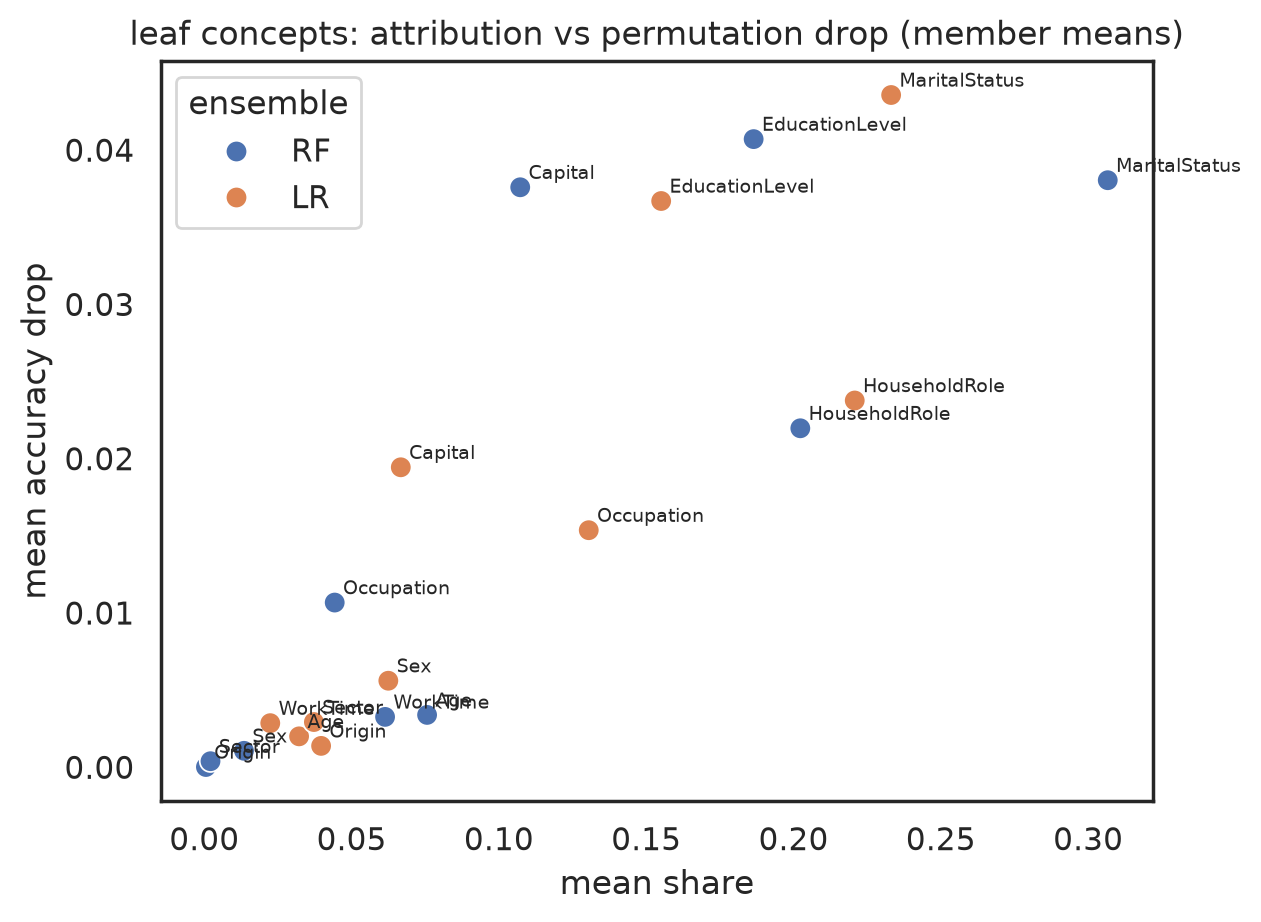
\includegraphics[width=0.6\textwidth]{faithfulness.png}
  \caption{Mean concept share vs.\ mean accuracy drop under concept permutation.}
  \label{fig:faith}
\end{figure}

%=====================================================================
\section{Discussion and limitations}\label{sec:discussion}
%=====================================================================

\paragraph{Summary of answers.}
\begin{description}
  \item[RQ1] Yes, members rely on the same concepts far above chance, and more so at the top ontology level. The
    hierarchy absorbs substitutions between correlated features (\concept{MaritalStatus} vs.\
    \concept{HouseholdRole}) into agreement on \concept{Family}.
  \item[RQ2] Prediction disagreement is accompanied by disagreement on the \emph{dominant} concept, not on the full
    ranking. Borderline \texttt{>50K} votes rely on \concept{Finance}/\concept{Education}, \texttt{<=50K} votes on
    \concept{Family}, \concept{Demographics}, working time and protected attributes.
  \item[RQ3] Trees concentrate their attribution and agree more on the dominant concept; LR members spread
    attribution and agree more on the full ranking.
\end{description}

\paragraph{Limitations.}
\begin{itemize}
  \item \textbf{Attribution is not reasoning.} Contributions show which features a member used for a sample, not
    why it was trained that way; the same caveat applies to the mapping-network justifications reviewed in
    RR1~\cite{ribeiro2021aligning}.
  \item \textbf{Absolute concept vectors} show how much a concept is used, not its direction: ``the
    \texttt{<=50K} camp relies more on \concept{Family}'' does not mean that \concept{Family} pushes it to
    \texttt{<=50K}.
  \item \textbf{Tree attribution method.} Saabas path credits are order-dependent and not Shapley
    values~\cite{lundberg2017shap}; Laplace smoothing changes the values at small nodes.
  \item \textbf{Correlated features.} \code{marital-status} and \code{relationship} are near substitutes, so leaf-level
    disagreement between them partly reflects which one a member happened to split on.
  \item \textbf{Small contested set.} The RF contested bucket holds only 190 samples.
  \item \textbf{One split, one seed.} All results use the official test split and \code{random\_state=42}; no
    variance over seeds is reported.
  \item \textbf{Hand-built ontology.} The hierarchy was derived from the EDA and supervisor review; a different
    grouping would change the top-level results.
\end{itemize}

\paragraph{Future work.} Repeat over several seeds and ensemble sizes; replace Saabas credits with TreeSHAP to
remove order dependence; use signed concept vectors to study direction; and use the \concept{ProtectedAttribute}
view as a constraint (e.g.\ retrain without \code{relationship}) to see whether agreement shifts to other concepts.

%=====================================================================
\appendix
\section{Reproducibility}
%=====================================================================
The project uses \code{uv} (Python 3.14) with \code{numpy}, \code{pandas}, \code{requests}, \code{rich},
\code{scikit-learn}, \code{scipy}, \code{owlready2} and \code{seaborn}. Reusable code lives in
\code{src/project\_acl/} (\code{data}, \code{preprocess}, \code{ontology}, \code{ensemble}, \code{concepts},
\code{log}); the analysis lives in five notebooks that run top to bottom.

\begin{lstlisting}
uv sync
uv run project-acl-data          # download UCI Adult into data/raw/
uv run project-acl-preprocess    # data/processed/adult.csv
uv run pytest                    # contribution sums, ontology coverage, metrics
uv run jupyter nbconvert --execute --inplace notebooks/0*.ipynb
\end{lstlisting}

\printbibliography

\end{document}
